%============================================================================
% tento soubor pouzijte jako zaklad
% (c) 2008 Michal Bidlo
% E-mail: bidlom AT fit vutbr cz
%============================================================================
% kodovaní: iso-8859-2 (zmena prikazem iconv, recode nebo cstocs)
%----------------------------------------------------------------------------
% zpracování: make, make pdf, make desky, make clean
% připomínky posílejte na e-mail: bidlom AT fit.vutbr.cz
% vim: set syntax=tex encoding=latin2:
%============================================================================
\documentclass[english,cover]{fitthesis} % odevzdani do wisu - odkazy, na ktere
% se da klikat \documentclass[cover,print]{fitthesis} % pro tisk - na odkazy se neda klikat
%\documentclass[english,print]{fitthesis} % pro tisk - na odkazy se neda klikat
%      \documentclass[english]{fitthesis}
% * Je-li prace psana v anglickem jazyce, je zapotrebi u tridy pouzit 
%   parametr english nasledovne:
%\documentclass[english]{fitthesis}
% * Neprejete-li si vysazet na prvni strane dokumentu desky, zruste 
%   parametr cover

% zde zvolime kodovani, ve kterem je napsan text prace
% "latin2" pro iso8859-2 nebo "cp1250" pro windows-1250, "utf8" pro "utf-8"
%\usepackage{ucs}
\usepackage[utf8]{inputenc}
\usepackage[T1, IL2]{fontenc}
\usepackage{url}
\usepackage{siunitx}
\usepackage{amsmath}
\usepackage{listings}
\usepackage[acronym,nonumberlist,nomain]{glossaries}
\usepackage[section]{placeins}
\DeclareUrlCommand\url{\def\UrlLeft{<}\def\UrlRight{>} \urlstyle{tt}}

%zde muzeme vlozit vlastni balicky


% =======================================================================
% balíček "hyperref" vytváří klikací odkazy v pdf, pokud tedy použijeme pdflatex
% problém je, že balíček hyperref musí být uveden jako poslední, takže nemůže
% být v šabloně
\ifWis
\ifx\pdfoutput\undefined % nejedeme pod pdflatexem
\else
  \usepackage{color}
  \usepackage[unicode,colorlinks,hyperindex,plainpages=false,pdftex]{hyperref}
  \definecolor{links}{rgb}{0.4,0.5,0}
  \definecolor{anchors}{rgb}{1,0,0}
  \def\AnchorColor{anchors}
  \def\LinkColor{links}
  \def\pdfBorderAttrs{/Border [0 0 0] }  % bez okrajů kolem odkazů
  \pdfcompresslevel=9
\fi
\fi

%Informace o praci/projektu
%---------------------------------------------------------------------------
\projectinfo{
  %Prace
  project=BP,            %typ prace BP/SP/DP/DR
  year=2015,             %rok
  date=\today,           %datum odevzdani
  %Nazev prace
  title.cs={Vizualizace elektrických signálů mozku},  %nazev prace v cestine
  title.en={Brain Signals Visualization}, %nazev prace v anglictine
  %Autor
  author={Ivan Ševčík},   %jmeno prijmeni autora
  %author.title.p=Bc., %titul pred jmenem (nepovinne)
  %author.title.a=PhD, %titul za jmenem (nepovinne)
  %Ustav
  department=UITS, % doplnte prislusnou zkratku: UPSY/UIFS/UITS/UPGM
  %Skolitel
  supervisor= Michal Košík, %jmeno prijmeni skolitele
  supervisor.title.p=Ing.,   %titul pred jmenem (nepovinne)
  %supervisor.title.a={Ph.D.},    %titul za jmenem (nepovinne)
  %Klicova slova, abstrakty, prohlaseni a podekovani je mozne definovat 
  %bud pomoci nasledujicich parametru nebo pomoci vyhrazenych maker (viz dale)
  %===========================================================================
  %Klicova slova
  keywords.cs={Klíčová slova v českém jazyce.}, %klicova slova v ceskem jazyce
  keywords.en={Klíčová slova v anglickém jazyce.}, %klicova slova v anglickem jazyce
  %Abstract
  abstract.cs={Výtah (abstrakt) práce v českém jazyce.}, % abstrakt v ceskem jazyce
  abstract.en={Výtah (abstrakt) práce v anglickém jazyce.}, % abstrakt v anglickem jazyce
  %Prohlaseni
  declaration={Prohlašuji, že jsem tuto bakalářskou práci vypracoval samostatně pod vedením pana ...},
  %Podekovani (nepovinne)
  acknowledgment={Zde je možné uvést poděkování vedoucímu práce a těm, kteří poskytli odbornou pomoc.} % nepovinne
}

%Abstrakt (cesky, anglicky)
\abstract[cs]{
Tato práce pojednáva o problematice zpracování a vizualizace mozkových signálů
a jejich využití pri analýze dat měřených pomocí EEG. 
Práce obsahuje úvod do anatomie mozku a povahy mozkové aktivity, který je pak
využit při popisu jedné z metod meření této aktivity, konkrétně EEG. Dále se práce
zabýva metodami zpracování signálů, především filtrací, a metodami vizualizace.
Rovněž je zde uveden prěhled předchozích rešení zabývajících se
vizualizací biosignálů, které sloužily jako výchozí představa při tvorbě konceptu 
vlastní aplikace.
Tato aplikace byla napsána v jazyce C++ s využitím knihovny Qt pro vytvoření 
multiplatformního grafického uživatelského rozhraní. Důležitým aspektem bylo
také využití rozhraní OpenGL, které umožnilo hardwarově akcelerovat vykreslování
a tím pádem dosáhnout uspokojivé překreslovací frekvence. Dále bylo využito několik
knihoven, ktére implementují načtení EEG dat ze souboru, rychlou Fourierovou transformaci,
matematické operace v 2D a 3D prostoru, a načítání 3D objektů ze souboru.
Implementace pak řeší několik problémů. V první řade je to vykreslování
2D a 3D modelů mozku a vizualizace mozkové aktivity nad těmito modely formou animovaných
elektrod. V důsledku
využití OpenGL bylo nutné pro tyto operace napsat příslušné shader programy, které
řídí grafickou kartu v procesu vykreslování. Aplikace obsahuje také prohlížeč 
mozkové aktivity ve formě vícenásobného grafu. U něj bylo nutné řešit vykreslování
velkého množství dat, které je počas EEG sezení naměřeno. To je řešeno decimací
signálu metodou, při které se z několika vzorků vybere maximum a minimum, která
jsou následně vykreslena. Tato metoda poskytuje výrazné zrychlení běhu aplikace
při zachování charakteristické křivky signálu. 
Protože EEG data sou ve své podstatě signály, bylo žádoucí poskytnout také metody
pro zpracování signálů přímo v aplikaci. Aplikace tedy podporuje filtraci signálů
pomocí dolní a horní propusti a dvojici váhovacích oken -- Hammingovo a Blackmanovo.
Implementace této části byla testována porovnáním výsledků různých konfigurací s
výstupem programu MATLAB, ve kterém byli vytvořeny shodné filtry.
Výsledná aplikace představuje nástroj pro analýzu mozkových signálů kombinující
prohlížení signálů s prostorovými vizualizacemi. Prostorová vizualizace poskytuje
přehledný způsob pro zkoumání průběhu všech signálů v čase a umožňuje snadnou 
vizuální identifikaci mozkové aktivity. Ta může být podrobněji analyzována právě pomocí
prohlížeče signálů. 
Aplikace zatím nepodporuje řadu žádaných funkcí, např. nahrávaní a zpracování signálů
v reálnem čase. Tyto nedostatky spolu s navrhovanými řešeními jsou uvedena v závěru práce.
Nicméně, součásna implementace poskytuje vhodný základ pro plánovaný budoucí vývoj.
}
\abstract[en]{
EEG is a non-invasive method for measuring brain activity that gives an important insight into mental processes. This work presents an application that serves as a visual EEG data analysis tool. The application concept was based on the existing work done in this field. The application combines signal display in form of a view composed of multiple charts with 2D and 3D visualizations that are helpful in recognition of particular brain activity. In addition, it implements convenient signal processing methods. The thesis is concluded by a summarization of accomplishments and future work's directions.
}

%Klicova slova (cesky, anglicky)
%\keywords[cs]{Sem budou zapsána jednotlivá klíčová slova v českém jazyce, oddělená čárkami.}
%\keywords[en]{Sem budou zapsána jednotlivá klíčová slova v anglickém jazyce, oddělená čárkami.}

%Prohlaseni
\declaration{Prohlašuji, že jsem tuto bakalářskou práci vypracoval samostatně pod vedením pana Ing. Michala Košíka. Uvedl jsem všechny literární prameny a publikace, ze kterých jsem čerpal.}

%Podekovani (nepovinne)
\acknowledgment{Týmto by som sa rád poďakoval svojmu vedúcemu Ing. Michalovi Košíkovi za odbornú pomoc a cenné rady pri vypracovaní bakalárskej práce.}

\makeglossaries

\begin{document}
  % Vysazeni titulnich stran
  % ----------------------------------------------
  \pagenumbering{Alph}
  \maketitle
  \pagenumbering{arabic}
  \setcounter{tocdepth}{1}
  % Obsah
  % ----------------------------------------------
  \tableofcontents
  
  % Seznam obrazku a tabulek (pokud prace obsahuje velke mnozstvi obrazku, tak se to hodi)
  % \listoffigures
  % \listoftables 

  % Text prace
  % ----------------------------------------------
  %=========================================================================
% (c) Ivan Ševčík, 2015

% Acronym definitions
\newacronym{eeg}{EEG}{Electroencephalography}
\newacronym{mri}{MRI}{Magnetic resonance imaging}
\newacronym{pet}{PET}{Positron emission tomography}
\newacronym{pc}{PC}{Personal computer}
\newacronym{cpu}{CPU}{Central processing unit}
\newacronym{gpu}{GPU}{Graphics processing unit}
\newacronym{api}{API}{Application programming interface}
\newacronym{sdk}{SDK}{Software development kit}
\newacronym{dft}{DFT}{Discrete Fourier transform}
\newacronym{fft}{FFT}{Fast Fourier transform}
\newacronym{dsp}{DSP}{Digital signal processing}
\newacronym{2d}{2D}{Two dimensional}
\newacronym{3d}{3D}{Three dimensional}
\newacronym{gui}{GUI}{Graphical user interface}

%Print the glossary
%\printglossaries
\glsunsetall

%TODO: articles and commas check, check, check..
%TODO: http://www.grammarbook.com/punctuation/commas.asp
\chapter{Introduction}
% Uvod do temy
A brain is a central organ of a human nervous system and as such it has a very
important role in almost every activity. However, its complexity makes it
difficult to study and understand. The rapid development of computers in recent
decades provided a partial solution to this problem as it allowed for mapping and
monitoring both a structure and an activity of brain with a high precision \cite{compForBrainStudy}.

% Aktualny stav, problemy
But raising interest in the \gls{eeg} technology and brain-computer interfaces also means
that there is an evident need for user interfaces and applications capable of
processing these signals for various purposes. One such purpose is visualization
that allows researchers and users to better comprehend measured data as these
are usually just binary values that may be represented as integer or decimal
numbers, therefore hard for humans to interpret. Another issue is that,
generally, users are not interested in raw values but in some features that the
signal carries, such as intensity at certain frequency or specific patterns that
represent a certain activity performed by a measured subject \cite{eegWaveFt}.

% Ciele
The goal of this work is to create an application implementing several
methods of the signal processing and the visualization, including classification by
frequency, charts showing waveform of measured signal in time domain, and both
a two and a three-dimensional model displaying brain activity. Another important
task will be to create an intuitive and clean, yet highly customizable graphical
user interface that will be responsive also for real-time signal inputs. The
application should, however, be able to process also large offline data measured
earlier without noticeable performance decrease.

% O com to tu je
The text is structured into chapters that start as a general theory and
progressively get more specific, concluded by an application concept and
implementation. In Chapter \ref{humanBrain}, a background information about brain
and methods for measuring its activity, specifically \gls{eeg}, is presented. Moving
on, Chapter \ref{appProcVis} provides required foundations of signal processing
and computer visualization. Chapter \ref{existSol} contains reviews of few existing
solutions in field that serve as an inspiration for this work. The concept for the application is
introduced in chapter \ref{concept} and eventually transforms into
implementation, which is described in Chapter \ref{implementation}.
 
\chapter{Human Brain} \label{humanBrain}
A human brain is a central unit of a human nervous system and has an important role in almost
every aspect of life. It performs both conscious tasks and an automatic operation
of vital organs, including breathing, maintaining blood pressure, and releasing
hormones. It also processes all the sensory inputs, such as odors, sounds, or light,
interprets them, and makes associations with representations preserved in memory.
\section{Brain Biology}
A biology of the human brain is complex and many mental processes are still not well understood. This section will, therefore, provide rather a very brief introduction to brain anatomy and communication mechanisms that are relevant for this work.
\subsection{Anatomy}
From an anatomy point of view, this work is interested primarily in a cerebrum because it is the part of the brain where an EEG activity occurs.
The cerebrum is the outermost structure of the brain. It is divided into two separate hemispheres that are
bridged by a bundle of fibers. The cerebrum is associated with a high-order
functioning and a control of a voluntary behavior. This includes thinking,
perceiving, planning, and language understanding. The cerebrum is covered with a
sheet of a tissue called cerebral cortex, which is further divided into regions called lobes
that are functionally differentiated. There are four lobes,
each with a different role \cite{brainFacts}: 
\begin{description}
	\item[Frontal lobe] is where initiation and coordination
	of motor movements take place, along with higher cognitive skills, such as
	thinking, planning, and organizing. It is also important for a personality and
	an emotional makeup.
	\item[Parietal lobe] is responsible for processing sensory
	inputs, attention, language and spatial orientation.
	\item[Occipital lobe]  helps to	process visual information and to assist with a recognition of shapes and colors.
	\item[Temporal lobe] is a region where auditory information is processed and
	information from other senses is integrated. It also has a role in the
	short-term memory and in learned emotional responses.
\end{description}
Figure \ref{fig:brainAnatomy} shows all the discussed structures on a model of the brain.

%TODO: footnote is on other page
\begin{figure}[htb]
	\centering
	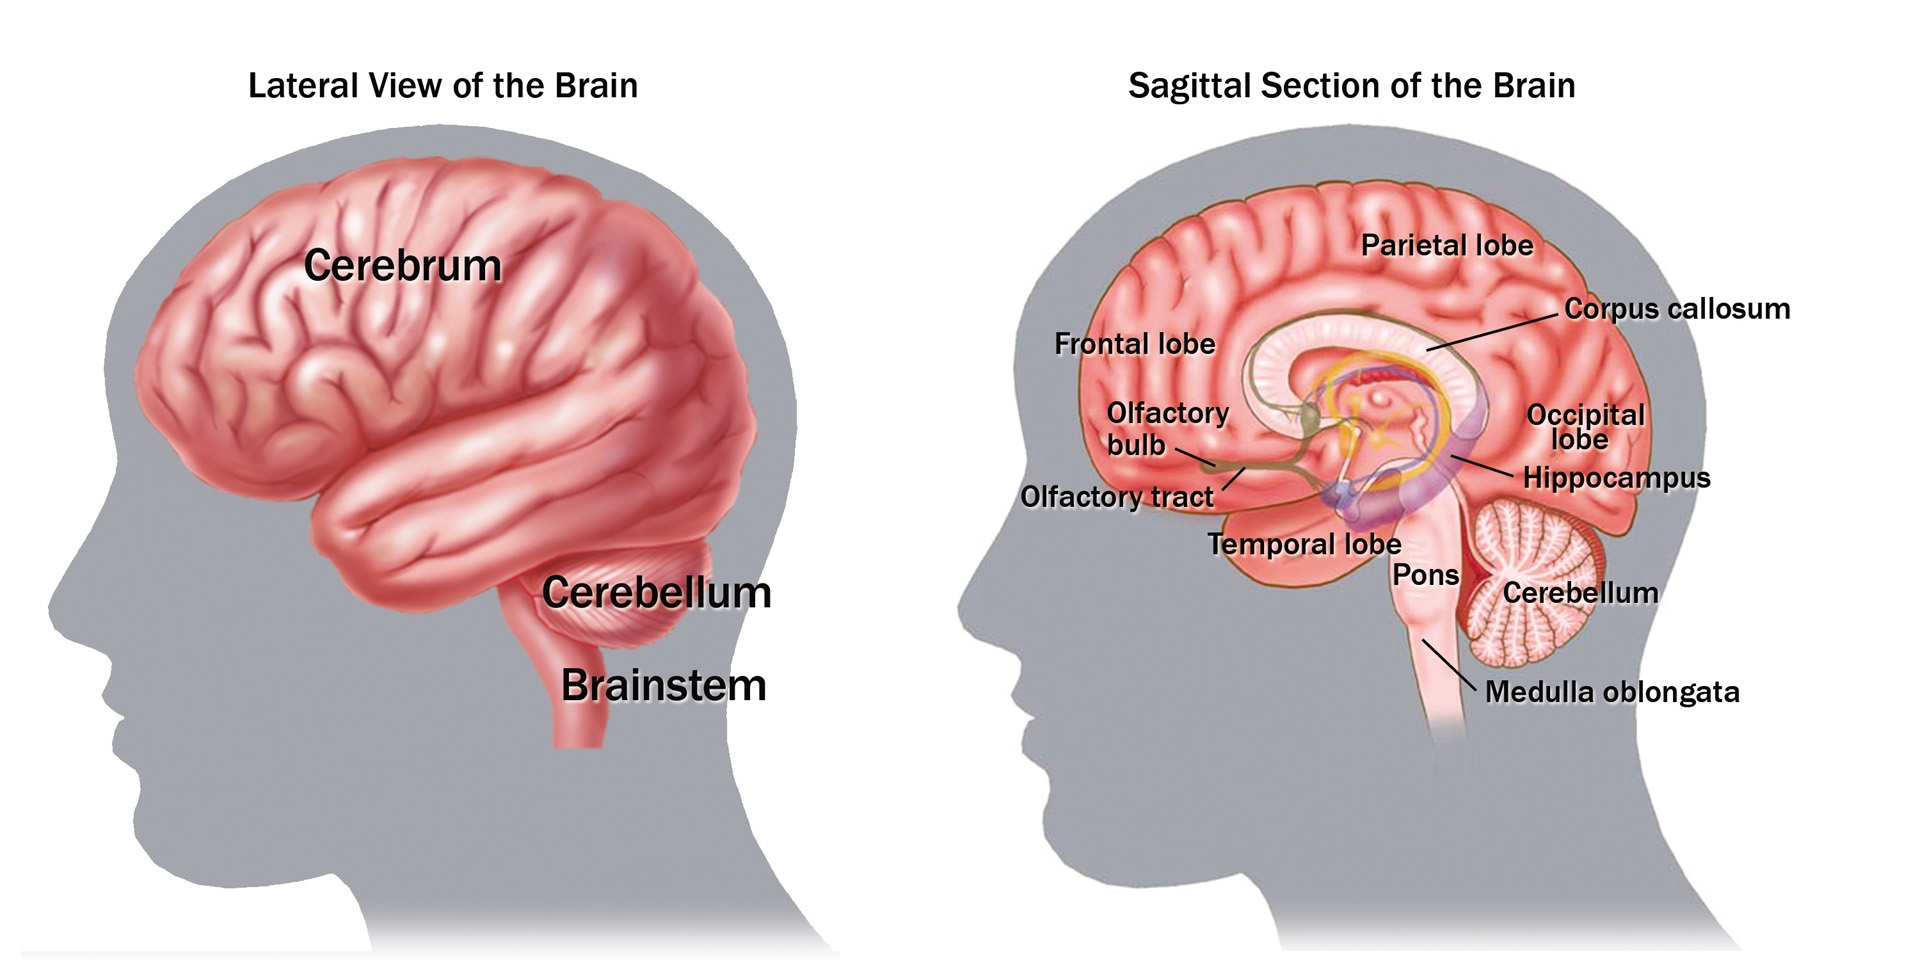
\includegraphics[width=1\linewidth]{fig/BrainAnatomy.jpg}
	\caption[Caption for LOF]{Brain anatomy\protect\footnotemark}
	\label{fig:brainAnatomy}
\end{figure}
\footnotetext{Image source \url{http://www.compelvisuals.com/wp-content/uploads/2013/12/BrainAnatomy-Newsletter.jpg}}

\subsection{Neurons}
The neural tissue is made of cells called neurons that communicate with each
other and represent basic working units of the brain.
The neuron consists of a cell body, dendrites and an axon, which can be seen in Figure \ref{fig:neuron}.
%TODO: footnote is on other page
\begin{figure}[htb]
	\centering
	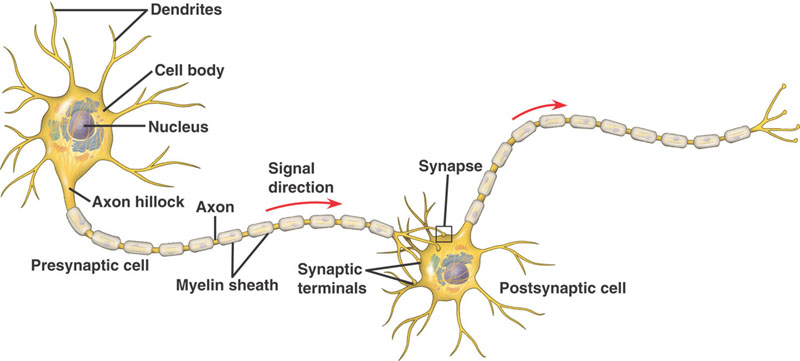
\includegraphics[width=0.8\linewidth]{fig/neuron2.jpg}
	\caption[Caption for LOF]{Neuron structure\protect\footnotemark}
	\label{fig:neuron}
\end{figure}
\footnotetext{Image source \url{http://2012books.lardbucket.org/books/beginning-psychology/section_07/6a3f0732c22683476ea201ffc5e428ad.jpg}}
The cell body contains a nucleus and a cytoplasm, and
produces peptides required for communication. Dendrites extend from the cell body and
receive signals from other neurons through synapses -- contact points where
axons of other neurons connect to dendrite. The axon is responsible for transmitting
electrical impulses outward from the neuron. These electrical impulses originate
from a sudden change of an electrical potential caused by a flow of ions through a cell
membrane. The change, also called an action potential, then passes along axon's
membrane and upon hitting its end releases neurotransmitters in nerve terminals.
The neurotransmitters diffuse across the synapse and bind to receptors on the surface
of a target cell's dendrite, which causes response in the target \cite{brainFacts}.

\section{Electroencephalography}
As has been presented, the nature of the human nervous system is electrical. When many neurons are active at the same time, the collective charge of ions is large enough to propagate as a wave to the surface of a brain or even to a scalp. Therefore, it is possible to observe a brain activity in underlying brain structures by measuring the variation of the surface electrical potential on the scalp. This is done by placing a conductive electrodes on the scalp and taking a measurement of the potential. The method just described is known as electroencephalography (\gls{eeg}) and it is a noninvasive way to monitor and study human brain. Earliest works used galvanometers and sophisticated techniques to take measurements \cite{eegHistory}, which has been since substituted by A/D converters and computers or other equipment for recording digital data. The recorded data can be then subjected to further digital signal processing (\gls{dsp}) \cite{eegClass}.

The main advantage of \gls{eeg} over other methods for monitoring brain activity, namely \gls{mri} and \gls{pet}, is speed as it can record responses
to a stimulus within fractions of a second \cite{eegFund}. Applications of \gls{eeg}
include:
\begin{itemize}
  \item Research -- monitoring of brain activity during cognitive and motoric tasks
  \item Medical -- diagnosis of brain diseases or confirmation of brain death 
  \item Human computer interaction -- execution of commands using brain activity  
\end{itemize}
Recently, the \gls{eeg} based devices were introduced also to a consumer market so users can monitor their brain activity at home, play simple games, or control toys using their thoughts\footnote{http://www.livescience.com/43250-mind-controlled-quadcopter.html}.

\subsection{Basic Principles}
The neural activity has mostly asynchronous nature. Because of this, it is impossible to measure or distinguish electrical activity of each neuron with \gls{eeg} as the individual potentials are combined by the time they propagate to the scalp.
What \gls{eeg} measures is a summated potential of a neural activity, which includes
a spontaneous electrical activity of the cerebral network and cortical responses to
external and internal events. The responses to events, characterized by their
onset latency and voltage amplitude, are referred to as \emph{event-related
potentials} and are either results of physical stimuli or behavioral responses \cite{bcComm}.

\subsection{Equipment for Taking EEG Measurements}
The setup used for encephalographic measurements usually consists of: 
\begin{itemize}
  \item Electrodes with conductive media
  \item Amplifiers with filters
  \item A/D converter
  \item Recording device
\end{itemize}
% Electrodes
Electrodes exist in various forms but this thesis will focus on
headsets and electrode caps, such as one displayed in Figure \ref{fig:eegCap}.
These caps usually consist of small discs serving as electrodes made
of a very conductive material, such as gold, silver, or stainless steel. The electrodes have long leads that can be plugged into an
amplifier \cite{eegFund}. The discs are in a direct contact with the scalp and can already
measure the electric potential produced by the brain. However, a conductive media in form of a
gel or a paste is often used to increase conductivity even more by lowering
contact impedance and improve readings at the lowest level. It also helps
electrodes to stick to the scalp surface so accidental shift in a position is less likely. There is also another type of electrodes that doesn't require application of gel. These are called dry electrodes and they use additional electronics to lower skin impedance, such as local impedance converting amplifier. Because of this, systems using dry electrodes are more bulky and more expensive but they don't require skin preparation and usage of gels that cause skin irritation \cite{dryElectrodes}. 

%TODO: footnote is on other page
\begin{figure}[htb]
	\centering
	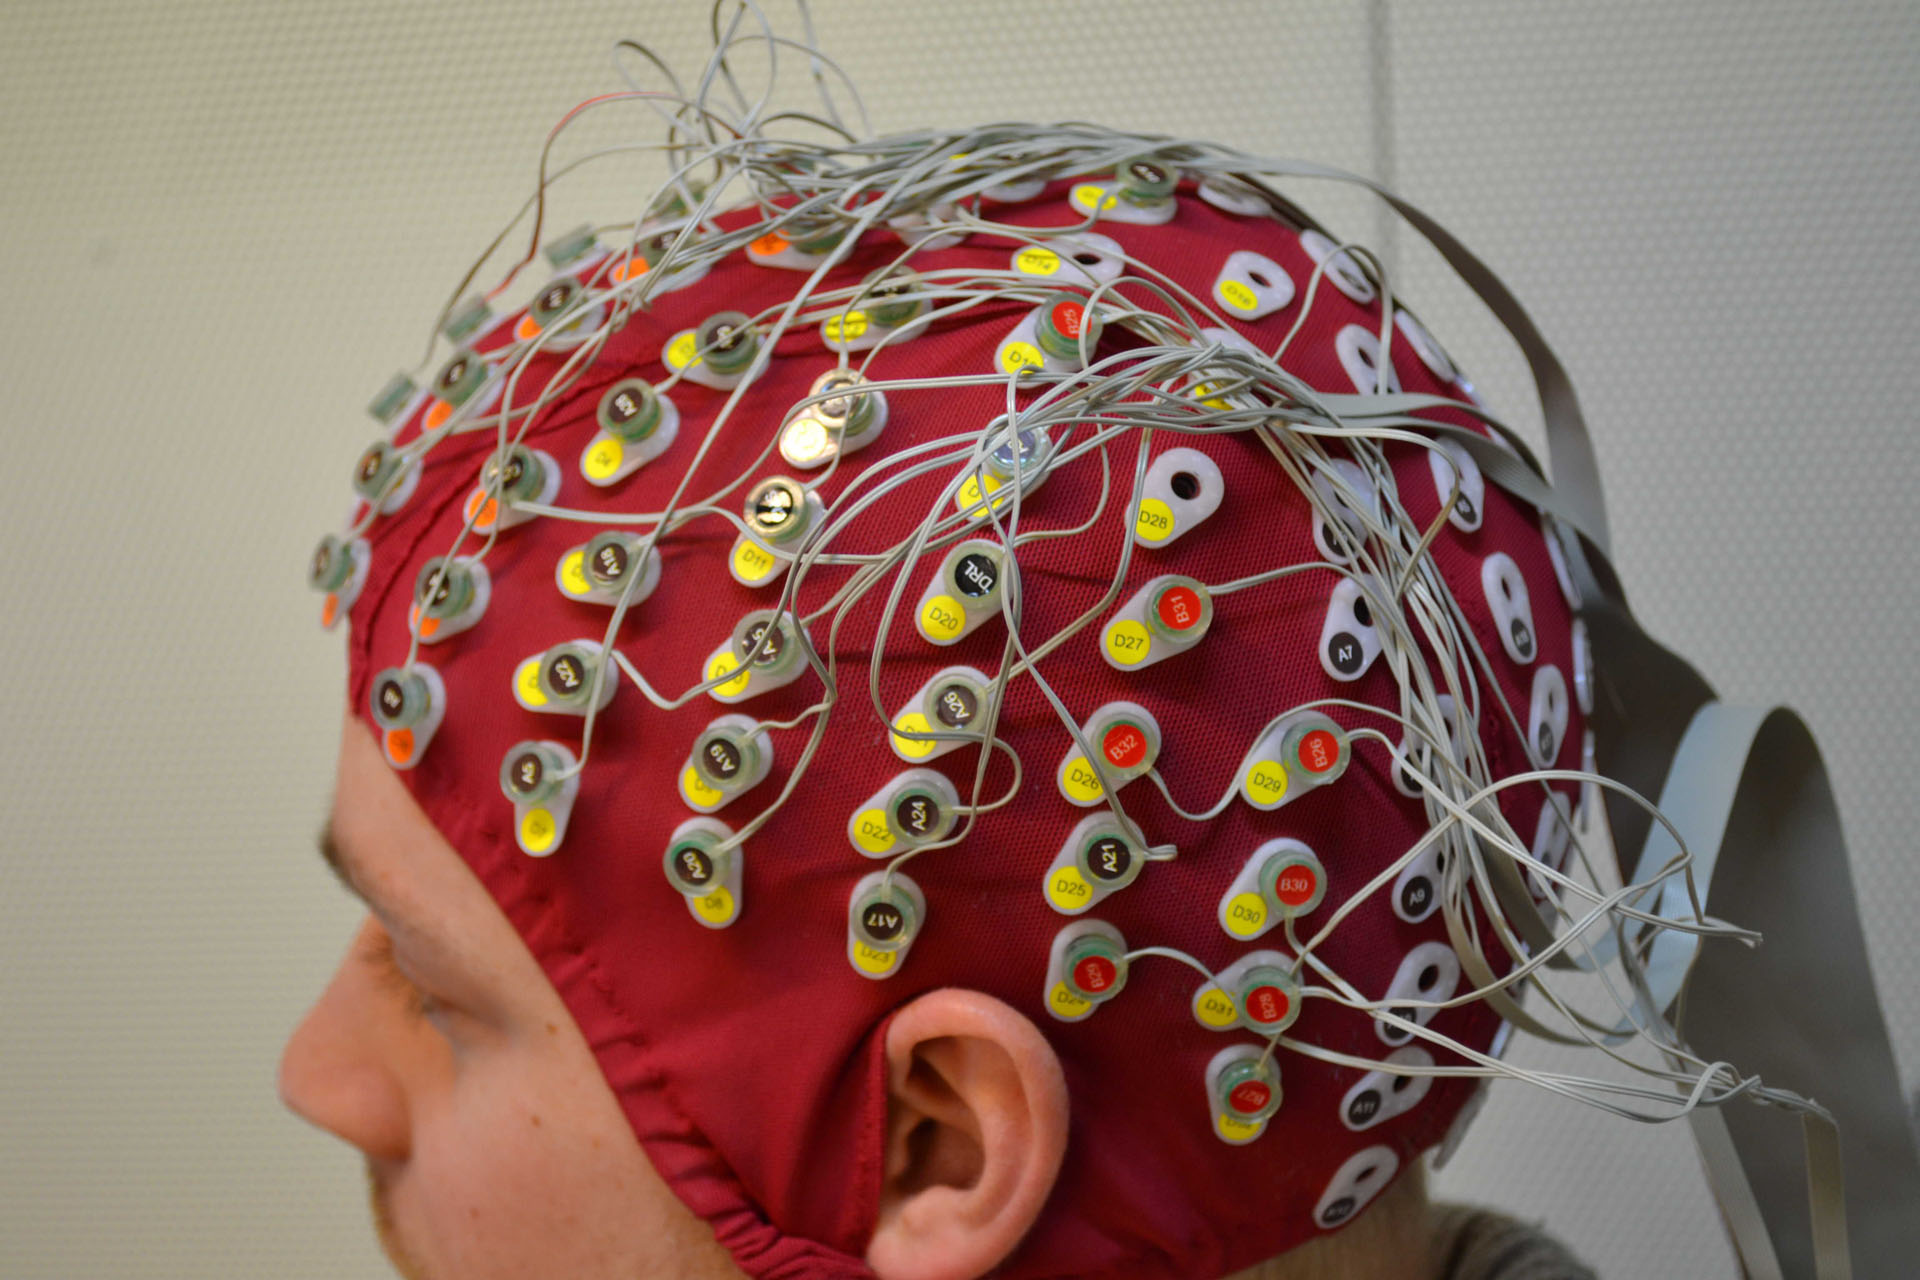
\includegraphics[width=1\linewidth]{fig/eegCap.jpg}
	\caption[Caption for LOF]{Electrode cap\protect\footnotemark}
	\label{fig:eegCap}
\end{figure}
\footnotetext{Image source \url{http://www.psychologie.uzh.ch/fachrichtungen/plasti/Labor/\gls{eeg}-03.jpg}}

% Cap
The electrodes are prepositioned on a silicon cap in locations according to
standardized placement system, which will be discussed later in this section.
This both speeds up the setup stage and allows for unified mapping of electrodes
to head surface. However, it fails to account for different shape and features of each
individual's head \cite{eegFund}. This problem is usually solved by involving a
method for finding \gls{3d} coordinates of electrodes on the head. Such methods
include using magnetic field digitizer or elaborate algorithms that can
calculate position of each electrode from few distance and angle measurements by
utilizing specific properties of standard placement system \cite{rapidPos}.

% Amplifiers
The strength of the signal measured by electrodes is in order of microvolts and
normally range from \SIrange{10}{500}{\uV} \cite{neuralAmp}. Therefore, an amplifier is needed to bring the amplitude to higher voltage levels that can be processed
by other electrical circuits and components. The requirements on amplifiers for
use with \gls{eeg} are high as they have to provide amplification only for the physiological
signal, which should not be distorted in any way, reject superimposed noise and
interference signals, and protect both the equipment and measured subject from
current surges. Amplifiers conforming to these requirements are known as
\emph{biopotential amplifiers}. \cite{biopotAmp}
% Filters
A band pass filter is then used to limit frequencies into a certain range of
interest. In some cases it may be already a part of the amplifier.
Another common filter is a notch filter, which can used to filter out noise
at frequency of a power line. Depending on a country, it may be set to
\SIlist[list-units = single, list-pair-separator = { or }]{50;60}{\Hz}
\cite{deltaCompNREM}. Such filter is only used if it is desirable to keep also
high frequencies because the interesting frequency bands usually lies bellow this
threshold and, therefore, a high pass filter would be sufficient.
% Trend in amplifier miniaturization
The trend in a development of neural recording devices is heading in a direction of
small and portable systems that can be used by patients with severe disorders in everyday life.
Consequently, energy efficient amplifiers are being designed lately that are very small, may run on battery for
long periods of time and dissipate only little heat \cite{neuralAmp}.

% A/D converter
An A/D converter unit is then used to convert analog values to digital
representation. The converter should have a resolution of at least 12 bits and
ideally 16 bits or more. With a high number of electrodes, analog multiplexers are
sometimes used to lower the number of necessary converter units at the expense
of a limited sampling frequency. The sampling frequency should be at least double of
the highest recorded frequency, for example the upper frequency limit of a
band pass filter. This is known as Nyquist-Shannon sampling theorem which is
fundamental for correct signal reconstruction without aliasing artifact. The
preferred sampling frequency is \SIrange{256}{400}{\Hz} \cite{guidDigEEG}.

% Recording device
Converted samples from A/D converters are then stored in a digital memory for further
processing which will be discussed later in this section \ref{sub:dataAnalysis}.
A recording device may be represented by a computer or by a
different piece of specialized equipment. The computer can be additionally
equipped with digital signal processor unit so that \gls{cpu} load is lower and can be
used for other tasks.

\subsection{Standard Electrode Placement}
\label{ssec:elPlacement}
% Uvod
The need for a standardized electrode placement was evident as early as 1947 when
the first International \gls{eeg} congress held place in London. Various methods of
standardization were proposed and this effort finally resulted in definition
of a 10-20 electrode system in 1958 by H.H. Jasper \cite{placeSys}. 
% Popis 10-20
This system consists of 21 electrodes placed evenly between certain landmarks
and the labels of electrodes are derived from cerebrum lobes above which the electrodes
are located. The first contour can be found by connecting inion and nassion.
Inion is a small protuberance at the back of a head and nassion is located just
above the bridge of a nose. The length of this line is measured and electrodes are
placed along it using following procedure. First electrode -- Fpz, is placed at
10\% of the contour length from the nassion. The electrodes Fz, Cz, and Pz are placed in this
order from front to back with spacing defined as 20\% of the length. Fz and Fpz are also
spaced by 20\%. Last electrode, Oz, is placed at 10\% of length from the inion
which equals 90\% of length from the nassion. It should be clear now why the system
is called 10-20. The rest of electrodes are placed in similar fashion.

% Popis 10-10
The 10-20 system offers only limited resolution but it was sufficient at the
time of its creation because the main limiting factor was technology. However,
with advances in electrode technology and miniaturization of electrodes, using more than
21 channels became feasible. Naturally, many laboratories sought to take advantage of the
higher resolution. With more electrodes than what is 10-20 model capable of
accommodating, first extension to the standard placement system was needed. The
extension, named 10-10 system, was proposed in 1985 and extended the number of supported
electrodes to 74. It uses additional coronal contours lying halfway between
original contours and combines the labels of these original contours to create
new label. For example, a contour lying between original contours F and C is labeled FC \cite{placeSys}. The positions of electrodes according to this
system are shown in Figure \ref{fig:system1010}. 

%TODO: footnote is on other page
\begin{figure}[htb]
	\centering
	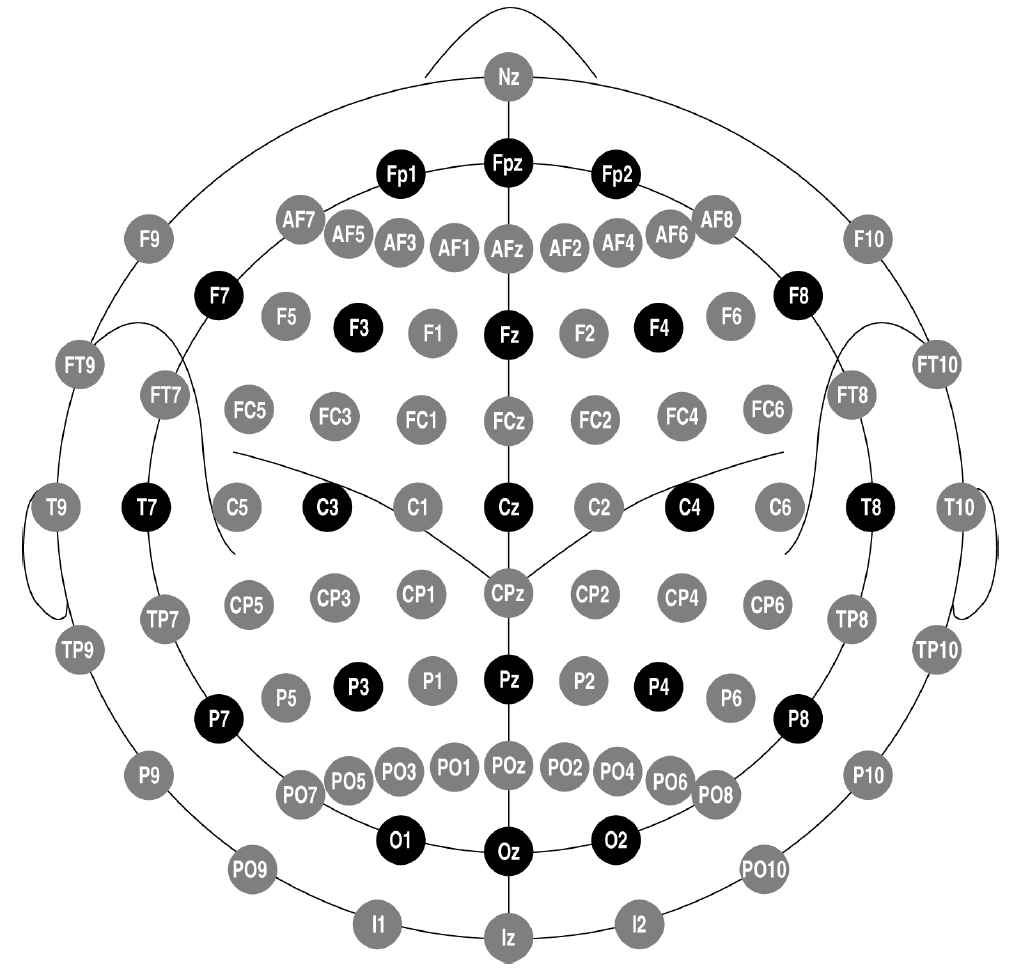
\includegraphics[width=1\linewidth]{fig/system10-10.png}
	\caption[Caption for LOF]{International 10-20 (black) and 10-10 (gray) system of \gls{eeg} sensor placement\protect\footnotemark}
	\label{fig:system1010}
\end{figure}
\footnotetext{Image source \cite{placeSys}}

% Popis 10-5
The 10-5 electrode placement system further extends the 10-10 system to allow an
even higher number of channels to be used as systems with over 128 channels are
not uncommon anymore and have become commercially available \footnote{\url{http://www.egi.com/company}}.
The total number of possible locations supported by 10-5 system is 345 \cite{placeSys}.
This system is in a proposition stage and is yet to be recognized as a standard.

%TODO: Delete if not needed
%\subsection{Measurement procedure}
%Before a measurement, the electrodes are cleaned thoroughly to remove any
%impurities that could have an impact on it. The skin is also cleaned from oils
%and brushed from dried parts. It is important to adhere to a strict hygiene as
%this might cause irritation and inflammation, and with repeated measurements may
%develop into an infection \cite{eegFund}. The subject is then seated comfortably
%to eliminate any unnecessary movement because it could spoil the measured data.
%Electrodes or an electrode cap are placed on subject's scalp and recording can begin.
%In case of a research oriented session, the subject is usually instructed to
%perform specific tasks such as imagining moving a certain part of a body, rotating
%an object in \gls{3d} space, or focusing on a specific area of a display device \cite{bcComm}. For other
%purposes, such as medical diagnosis, subjects may be monitored while laying on
%their back with closed eyes or during sleep.

\subsection{Data Analysis} \label{sub:dataAnalysis}
The recorded data are subject to further processing using numerical filters and
transforms in order to improve the signal-to-noise ratio and extract desired signal features. 
% Clasification by frequency band
One such feature is brain activity at a certain frequency. The frequency of brain
waves range from \SIrange{1}{150}{\Hz}. This range can be further divided
into six common categories \cite{dominantF}:
\begin{itemize}
  \item Delta waves -- below 4 Hz
  \item Theta waves -- between 4 and 8 Hz
  \item Alpha / Mu waves -- between 8 and 13 Hz
  \item Beta waves -- between 13 and 30 Hz
  \item Gamma waves -- between 30 and 80 Hz
  \item High gamma waves -- above 80 Hz
\end{itemize}
A healthy person exhibits brain waves mostly in the first four categories. Each
band is related to a certain group of an activity in the brain \cite{dominantF}. Delta waves are normally
distributed over scalp and may be significant during deep sleep, in childhood, or
in serious organic brain disease \cite{eegClass}. Theta waves are related to
cognitive tasks such as working memory and error monitoring tests. Alpha power
is increased during inattention and lack of visual input, therefore related to
perception. Mu power, on the other hand, is linked to movement and is decreased
when person performs a motor action. The distinction between alpha and mu waves
is made by considering the location of the electrode. While alpha waves form at the
back of the scalp, mu waves can be observed in a strip of brain from ear to ear
called motor cortex. Beta waves are low amplitude, high frequency waves
that have power reduced at the onset of a movement, rebound if the movement is
sustained, and are enhanced if the movement is suppressed. Finally, peaks in gamma and high gamma bands are observed in some brain areas but this activity varies too much across individuals to be reliably characterized \cite{dominantF}.

% Classification by pattern
Another set of features are patterns, such as those of event related potentials, that represent a certain activity more clearly than classification by frequency. Event related potentials are electrical brain responses time-locked to a physical stimuli or behavioral responses and characterized by their voltage amplitude and their latency in relation to stimulus onset \cite{bcComm}. For example, the imagined movement of
finger can be distinguished from imagined movement of leg with this method. The
classification accuracy is, however, highly individual and a classification
system usually needs a tuning or a calibration process for each user \cite{bcComm}.
Common approach to this problem is to train a neural network that can classify
patterns in brain waves with accuracy high enough for normal usage.

\chapter{Approaches to Signal Processing and Visualization} \label{appProcVis}
Once the data from electrodes have been recorded they can be processed and visualized according to chosen analysis method. This chapter will provide information about methods that are commonly used for processing signals and visualization of such data. A more specific terminology will used in the following text. The term signal processing will be from now on restricted to digital signal processing as the processing will be performed on software level. Likewise, the term signal will be restricted to a discrete-time signals represented by a sequence of numbers. 

\section{Signal Processing} \label{sec:sigProc}
In general, signal processing is concerned with representation, transformation, and manipulation of signals and the information they contain. For example, it can be used after an EEG measurement to ease analysis of recorded data by filtering out noise and selecting signal features, as presented in Section \ref{sub:dataAnalysis}. This section, therefore, provides general information about
methods of signal processing and specific implementation details are discussed in Section \ref{sec:implFIRfilters}. 

\subsection{Discrete Fourier Transform}
Discrete Fourier transform (\gls{dft}) is an operation that produces a corresponding frequency spectrum for any given sequence of numbers. Formally the \gls{dft} is defined by Equation \ref{eq:DFT} where the sequence $x(n)$ represents the input, usually a signal \cite[p. 401]{DSP3}. 

\begin{equation}
\label{eq:DFT}
	X(k) = \sum\limits_{n=0}^{N - 1}x(n)e^{-2 j \pi k n /N} \qquad 0 \leq k \leq N-1
\end{equation}

The product of the \gls{dft} is a new sequence $X(k)$ of complex numbers equally spaced in frequency domain. Each number represents a sample in the frequency spectrum. Because the numbers are equally spaced, each sample belongs to a certain frequency interval that is often referred to as a frequency bin. A bin resolution, that is the length of each frequency interval, can be determined through Equation \ref{eq:DFTres} where $f_s$ is the sampling frequency of the input signal. 

\begin{equation}
\label{eq:DFTres}
bin_{res} = \frac{f_s}{N}
\end{equation}

The direct computation of \gls{dft} is inefficient and contains repeating, and therefore redundant, operations. Because of that, a more efficient algorithm called \emph{fast Fourier transform} (\gls{fft}) is used in practical applications. The \gls{fft} algorithm takes advantage of symmetry and periodicity to reduce number of operations needed to compute the result. The number of complex multiplications can be used as a criterion when comparing the efficiency of \gls{dft} and \gls{fft}. Indeed, while \gls{dft} requires $N^2$ multiplications, the \gls{fft} algorithm requires only $(N/2)\,log_2N$ multiplications to produce the exactly same results. For example, the speed is improved $204.8$ times for a 1024 point \gls{dft} \cite[p. 459]{DSP3}.

\subsection{Filters in General}
A filter in the broadest context is any system that modifies certain frequencies relative to others. For the purposes of this thesis the term filter can be narrowed to a system that passes certain frequency components and totally rejects others \cite[p. 439]{DSP}. All the discussed filters will be causal. A system is causal, if for every choice $n_0$, the output sequence value at the index $n = n_0$ depends only on the input sequence values where index $n \leq n_0$ \cite[p. 21]{DSP}. The stability of filters will be also discussed in section \ref{ssec:FIRandIIR}. A system is stable if and only if every bounded input sequence produces a bounded output sequence. The input $x[n]$ is bounded if there exists a fixed positive finite value $B_x$, such that \cite[p. 21]{DSP}
\begin{equation}
	|x[n]| \leq B_x < \infty\text{,\qquad for all n.}
\end{equation}
The system is stable if for each bounded input there exists a fixed positive finite value $B_y$, such that \cite[p. 22]{DSP}
\begin{equation}
	|y[n]| \leq B_y < \infty\text{,\qquad for all n.}
\end{equation}

The filtering can be performed as convolution of the input signal with filter's impulse response in time-domain. Another, equivalent method is to first perform \gls{dft} for the input signal, multiply the obtained spectrum with filter's frequency response and perform an inverse \gls{dft}. 

\subsection{FIR and IIR Filters}
\label{ssec:FIRandIIR}
One of the most important decisions when considering the use of filters is the choice between finite and infinite impulse-response filters. They are two fundamentally different groups of filters with many differences, some of which will be discussed. The major difference between the systems can be seen from difference equations \ref{eq:FIRsystem} and \ref{eq:IIRsystem} \cite[p. 500]{DSP3}. While the FIR system uses only current and past input values, the input to the IIR system includes also previous output values.

\begin{align}
	\text{FIR system\qquad} &y(n)= \sum\limits_{k=0}^{M-1}b_kx\,(n-k) \label{eq:FIRsystem}\\
	\text{IIR system\qquad} &y(n)= -\sum\limits_{k=1}^{N}a_ky\,(n-k) + \sum\limits_{k=0}^{M}b_kx\,(n-k) \label{eq:IIRsystem}
\end{align}

Another difference between the FIR and IIR system involves stability. The FIR systems are inherently stable from the definition but a great care must be taken in order to design a stable IIR system. The IIR systems also suffer from limited precision of numbers in a digital representation. Therefore, an error accumulates over time due to the feedback. 

Considering the stated properties of both filter types it was chosen to further use only FIR filters as they are more suitable for EEG data processing. This claim is further supported by frequent use of FIR filters in other EEG related works, for example \cite{deltaCompNREM} and \cite{eegClass}.

\subsection{Low-pass and High-pass FIR Filters}
A low-pass filter is a system that ideally passes only frequencies below a specified threshold called cutoff frequency $f_c$. Accordingly, a high-pass filter is a system that passes only frequencies higher than the threshold and attenuates the others \cite[p. 331]{DSP3}. 

The filter is created by finding the coefficients $b_k$ for Equation \ref{eq:FIRsystem}. This can be done in general by designing the desired frequency response in frequency domain and using inverse Fourier transform to obtain filter's impulse response $h(n)$ which represents the coefficients. However, the low- and high-pass filters are so common that the impulse response can be obtained using equations \ref{eq:lowPass} and \ref{eq:highPass} where $\omega_c = 2 \pi f_c$ and $M$ is the filter's length \cite[p. 472]{DSP}.

\begin{align}
\text{Low-pass\qquad} & h(n) = \begin{cases}
\frac{\sin \left( w_c \left( n - M / 2 \right) \right)}{\pi \left( n - M / 2 \right)} & \  \text{,if} \quad n \neq M / 2 \\[0.2em]
2 f_c & \  \text{,if} \quad n = M / 2
\end{cases} \label{eq:lowPass}\\[1em]
\text{High-pass\qquad} & h(n) = \begin{cases}
-\frac{\sin \left( w_c \left( n - M / 2 \right) \right)}{\pi \left( n - M / 2 \right)} & \  \text{,if} \quad n \neq M / 2 \\[0.2em]
1 - 2 f_c & \  \text{,if} \quad n = M / 2
\end{cases}\label{eq:highPass}
\end{align}

\subsection{Window Functions}
In general, the filter's impulse response obtained through inverse Fourier transform is infinite in length. Therefore, it must be truncated at some point, say at $n = M-1$, to yield the FIR filter of length $M$ \cite[p. 624]{DSP3}. The truncation is equivalent to multiplying the infinite impulse response by a rectangular window  which is defined by Equation \ref{eq:rectWind}.

\begin{equation}
\label{eq:rectWind}
w(n) = \begin{cases}
1 &\qquad 0 \leq n \leq M-1\\
0 &\qquad \text{otherwise}
\end{cases}
\end{equation}

However, such truncation produces undesired effects in the filter's frequency response. For example, let's consider an FIR low-pass filter with a cutoff frequency $f_c=\SI{0.4}{\Hz}$ and length $M=31$.
\begin{figure}[htb]
	\centering
	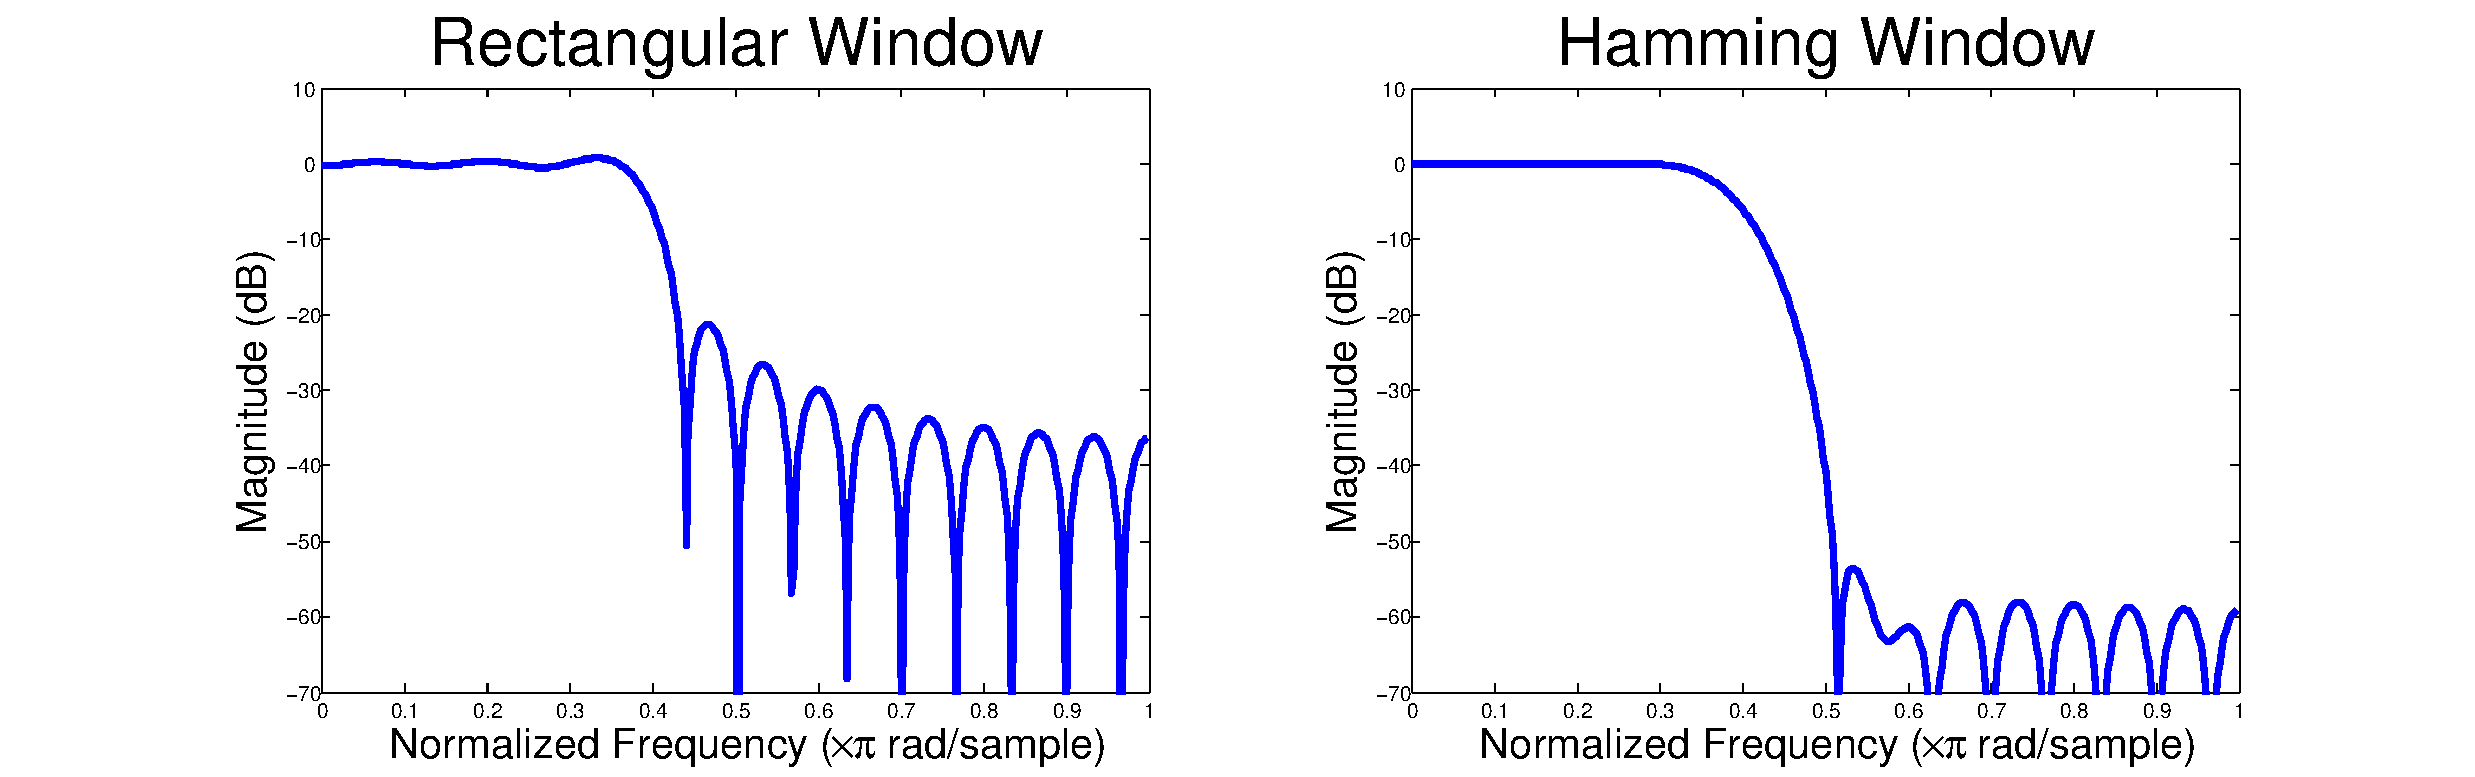
\includegraphics[width=1\linewidth]{fig/filterRiples.pdf}
	\caption{Comparison between filters with Rectangular and Hamming window}
	\label{fig:filterRiples}
\end{figure}
The left graph in Figure \ref{fig:filterRiples} depicts the frequency response of such filter after truncation. It can be seen that the gain at frequencies below cutoff moderately fluctuates and also that the attenuation at frequencies above cutoff is relatively small. The graph on the right side shows the frequency response for the exact same filter but the truncation was done using Hamming window. Clearly, the fluctuations are much smaller, almost invisible at this level of detail. Also, the filter better attenuates undesired frequencies. However, this comes at a cost of a longer transition to reach the stop band. While the filter with rectangular window reaches the stop band at frequency little over \SI{0.4}{\Hz}, the filter using Hamming window gets to the stop band at approximately \SI{0.5}{\Hz}. This is because the window attenuates data at its edges. Decreasing width in the time domain increases uncertainty in the frequency domain, which is represented by a filter response that has a shallower transition band stretching farther from the cut off frequency. Therefore, a choice must be made but the advantages of using window function usually outweigh the disadvantages.

The window function in essence weighs samples entering the filter so that transition into truncated area is smooth rather than sudden as in the case of rectangular window. The Equation \ref{eq:hammWind} defines the already discussed Hamming window and Equation \ref{eq:blackWind} defines another commonly used Blackman window \cite[p. 626]{DSP3}. The definitions are only for $0 \leq n \leq M-1$ as the rest of the impulse response is still truncated.

\begin{align}
\text{Hamming window\qquad}& w(n) = 0.54 - 0.46\cos \frac{2 \pi n}{M -1} \label{eq:hammWind}\\
\text{Blackman window\qquad}& w(n) = 0.42 - 0.5\cos \frac{2 \pi n}{M - 1} + 0.08\cos \frac{4 \pi n}{M - 1} \label{eq:blackWind}
\end{align}

\section{Data Visualization Methods}
So far, only methods for measuring and processing data have been
discussed but the primary goal of this thesis is to visualize them. Therefore, this section will discuss methods of data visualization using PC and common
display devices such as monitors and screens, and how these visualizations can
be used to help humans analyze data more easily.

\subsection{2D Representations}
Display devices and other media used for presenting information have mostly
two-dimensional nature. This has great implications for how the data are usually
visualized and manipulated. The most natural representations are those that are
already organized spatially as two-dimensional, without need for any projections
and mappings. It is still possible to add a next dimension of information through usage of
colors, different shapes and sizes, but the diagram layout remains two-dimensional. The most commonly used diagrams are based on
graphs and charts, although schematics and maps are also popular.

The graph is a type of diagram made of interconnected objects. The connection
may be represented by a line or curve which may be directed, meaning that it
goes only one way. Graphs are usually used for visual representations of data
where individual entities and their relations can be recognized, for example a
network of roads between cities, but they are also useful for displaying
hierarchies.

The chart is a visual representation of data useful for plotting, categorizing,
and showing trends. It may come in many forms, like bars or lines drawn in an
area designated by axes with scales, or slices of a pie. It is important to choose
the most suitable one, so that the most significant fact stands out.

\subsection{3D Models}
The world and objects within it are perceived by humans as three-dimensional
and, therefore, it is preferable to use three-dimensional representations of
objects called \gls{3d} models. However, there is lack of technology for displaying
such representations truly three-dimensionally, with holograms being the most
advanced one. Because of that, the models must be projected into two dimensions
so that they can be displayed using existing devices. This is done using
projection matrices during process called rendering. The two most common
projections are orthogonal and perspective.

There are multiple ways to create the \gls{3d} model. It is possible to scan real
world objects by various means, such as tomography and optical surface imaging.
Another method is to use special modeling software and reconstruct the model from basic
primitives. The model may have defined volume using volumetric or voxel
representations, or it can be just a surface of an object which is usually
represented by a mesh. The mesh is a collection of points in \gls{3d} space called vertices
which are interconnected to form basic primitives, like triangles and polygons.

\section{Programmable Graphics Pipeline}
\label{sec:pipeline}
A graphics pipeline represents the process of rendering and its stages. The
input data in form of vertices, colors, and other information are passed to the
first stage which processes and passes them down the pipeline to another stage.
The result of the final stage is rendered image of a scene. Before a programmable
pipeline was developed, programmers could only use vendor defined operations and
combine them to create their application. That imposed certain constraints on
what could be done, for example the number of light sources was limited. This approach
was called a fixed pipeline because the action performed by each stage was fixed and could be only modified through parameters
or states. With introduction of the programmable pipeline, it was possible for
programmers to step into the rendering process in several places and define their
own techniques. The custom programs that have become part of pipeline are called
shaders. 
\begin{figure}[htb]
	\centering
	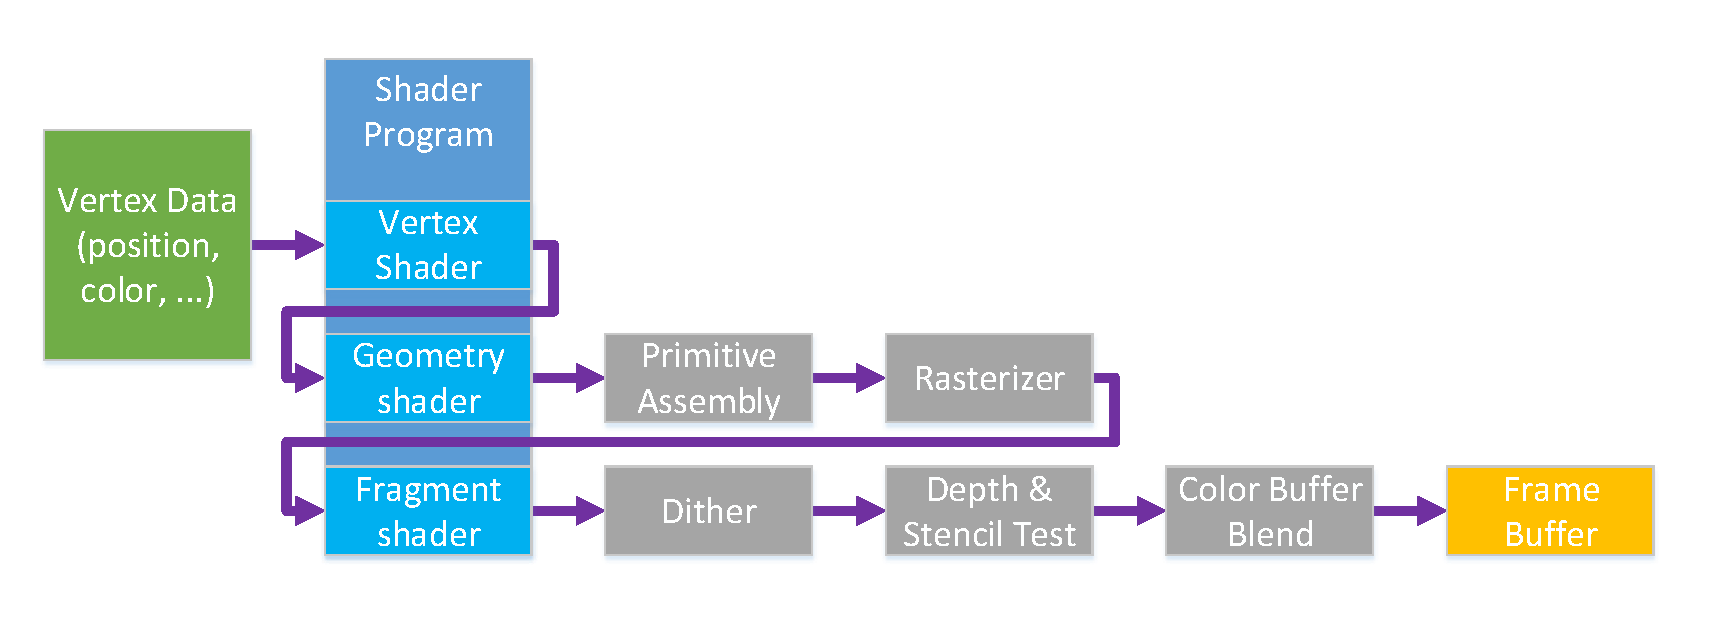
\includegraphics[width=1\linewidth]{fig/OpenGLpipeline.pdf}
	\caption{OpenGL 3.3 programmable graphics pipeline \cite{OpenGL}}
	\label{fig:OpenGLPipeline}
\end{figure}
The Figure \ref{fig:OpenGLPipeline} displays an OpenGL graphics pipeline \cite{OpenGL}. The three most important types of
shaders with respect to their position in the pipeline will be presented in following text. The terminology used in this section complies with OpenGL but the basic principles are similar for most of the graphics card APIs. For example, OpenGL shader programs are written OpenGL Shading Language (GLSL) and DirectX shader programs are written in High Level Shading Language (HLSL), both of which are derivatives of C language and provide similar features. A good introductory tutorial to modern OpenGL can be found at \url{http://www.opengl-tutorial.org/}.

\subsection{Vertex Shader}
A vertex shader is at the very beginning of the graphics pipeline, just after the primitive processing. It allows properties of vertices to be modified before they enter the geometry shader or the primitive assembly stage. The input to vertex shader is
single vertex with all the related information. Typical usage of this stage consists
of applying projection and transformation matrices, performing Gouraud shading \cite{goraud}, and controlling particle effects.

\subsection{Geometry Shader}
A geometry shader, if present, is executed right after the vertex shader but instead
of working with isolated vertices, it works with whole primitives like points,
lines and triangles. It may perform transformation from one type of primitive to
another and also emit completely new geometry. For example, it is possible to
have as input only one point and output may be a circle with that point as a
center. The circle can be made of varying number of triangles, depending on how far from camera
the point was. This not only saves time-expensive transport operation between
\gls{cpu} and \gls{gpu}, but also optimizes performance by dynamically lowering details.

\subsection{Fragment Shader}
A fragment shader works with individual pixels. However, the three-dimensional information have
not been discarded yet and is accessible during processing. This allows
three-dimensional effects, such as Phong shading \cite{phong}, to be applied at the finest level. The output
of this program is a single color that will be displayed by that specific pixel.

\chapter{Overview of Existing Solutions}
\label{existSol}
This chapter analyzes existing solutions focusing on their user interface, features, extensibility and intuitiveness. The work of other individuals or companies can serve as a source of inspiration when creating new application with similar purpose. It is possible to identify good ideas, which can be reused, by analyzing their solution.  

\section{Emotiv}
Emotiv is a company specializing in the area of \gls{eeg} devices for consumer market.
The product of the company is a headset accompanied with basic software and additional software can be bought or downloaded for free through a store
separately. On one side, the store allows the developers to create new
applications independently but as a result, there is a lack of a single, unified
user experience. This is caused not only by different styles the authors of each
application are using, but also because each application has its own set of
settings, controls, and displays, many of which are duplicated between
applications. For example, a chart with signals from electrodes is included in
both TestBench and \gls{3d} brain activity map applications. There is also another
brain activity map that displays each frequency band in \gls{2d}. The settings,
such as gain factor and buffer size, are not shared in any way between the
applications, resulting in different behavior which can be quite confusing.
However, the focus on ordinary computer users can be felt as the applications
are visually appealing and user-friendly. The TestBench and 3D activity map are displayed in figures \ref{fig:emotivTest} and \ref{fig:emotiv3d} respectively. 

%TODO: footnote is on other page
\begin{figure}[htbp]
	\centering
	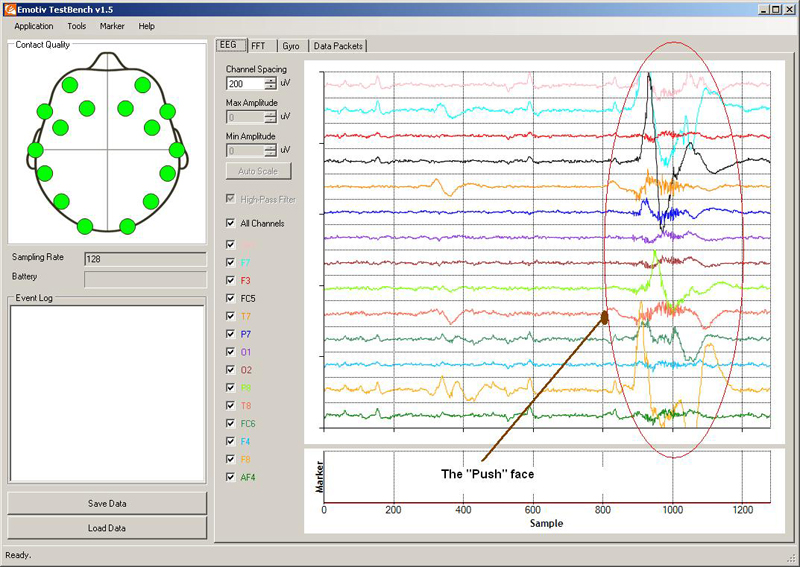
\includegraphics[width=0.8\linewidth]{fig/emotivTest.jpg}
	\caption[Caption for LOF]{Emotiv TestBench\protect\footnotemark}
	\label{fig:emotivTest}
\end{figure}
\footnotetext{Image source \url{http://common.ziffdavisinternet.com/util_get_image/22/0,1425,sz=1&i=221770,00.jpg}}

%TODO: footnote is on other page
\begin{figure}[htbp]
	\centering
	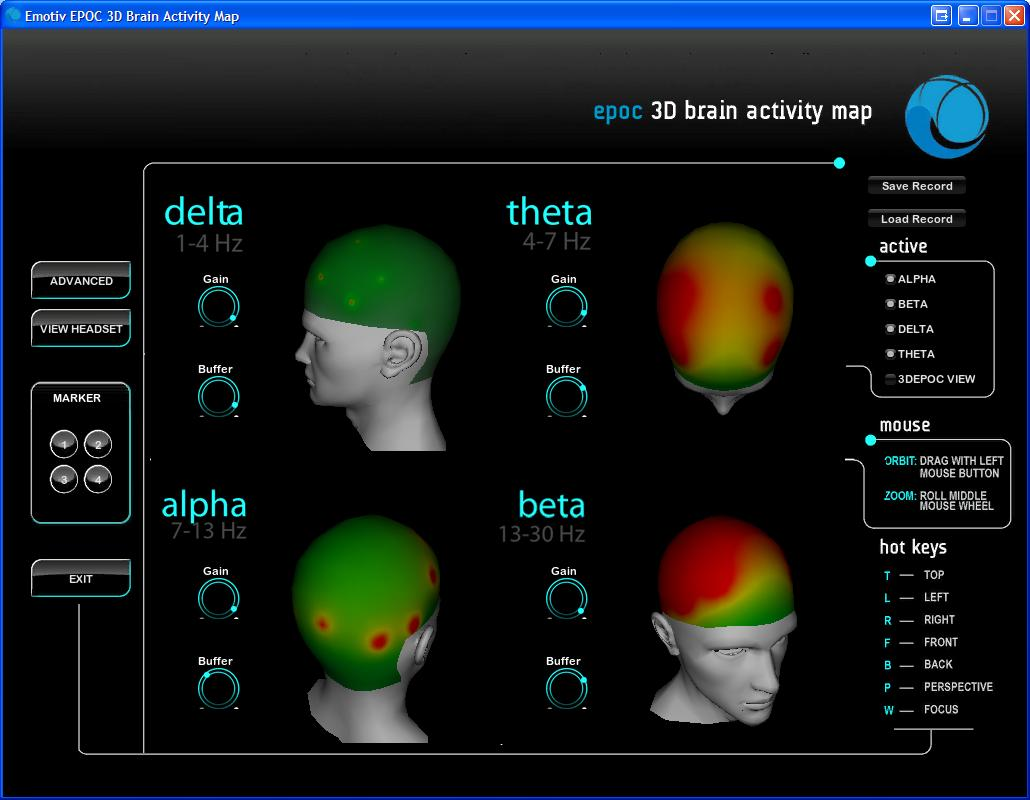
\includegraphics[width=0.8\linewidth]{fig/epoc3d.jpg}
	\caption[Caption for LOF]{Emotiv 3D brain activity map\protect\footnotemark}
	\label{fig:emotiv3d}
\end{figure}
\footnotetext{Image source \url{https://emotiv.com/upload/iblock/801/mainscreen.jpg}}

Feature-wise, the applications are ranging from visualization software and data
importers to games. One important feature that seems to be missing from most of
the applications is lack of any control of time, meaning they are only able to
display current values. It was only observed in the TestBench application. This is a very limiting factor for data analysis, as one of
basic tasks is comparing data. Being able to do so between two or more
moments in time is often desirable. The \gls{sdk} for creating new applications
is freely available, so anyone can start developing.

Currently, the company offers two options -- 14 channels EPOC and 5 channels Insight
headsets. These headsets come with built-in amplifiers, filters and A/D
converters, and communicate wirelessly with \gls{pc} through bluetooth.

\section{Svarog}
Svarog is an acronym that stands for Signal Viewer, Analyzer and Recorded on GPL. 
It is intended for use as an advanced analysis tool capable
of both online and offline signal viewing and processing. The data may be in any
data format as long as SignalML description is provided.

The application offers only basic visualization methods. Main GUI element
visible after starting the program is a chart with \gls{eeg} waveforms. It allows a user to:
\begin{itemize}
	\item Modify the amplitude range, time scale and amount of space between signals.
	\item Zoom in and out by reducing the number of displayed signals. 
	\item Select part of a signal spanning one or multiple electrodes.
	\item Perform \gls{fft} and show frequency spectrum for a segment of signal in superimposed window as shown in Figure \ref{fig:svarog}.
\end{itemize}
An interesting element is a time-frequency map that is
used for presenting results of a matching pursuit algorithm, which is one of the available
processing tools. Time is plotted on a horizontal axis, frequency on a vertical axis and
amplitude is represented by a color in a range from blue to red. However, there is
no brain or electrode map, or any other visually appealing elements.

The GUI is sometimes cluttered with too many options, which could have been
hidden in some advanced view, but overall is clean, quite customizable, and
informs a user about progress of operations. It also allows auxiliary
signal plots to be created, which are useful for signal comparison. Svarog is implemented in Java.

\begin{figure}[htb]
	\centering
	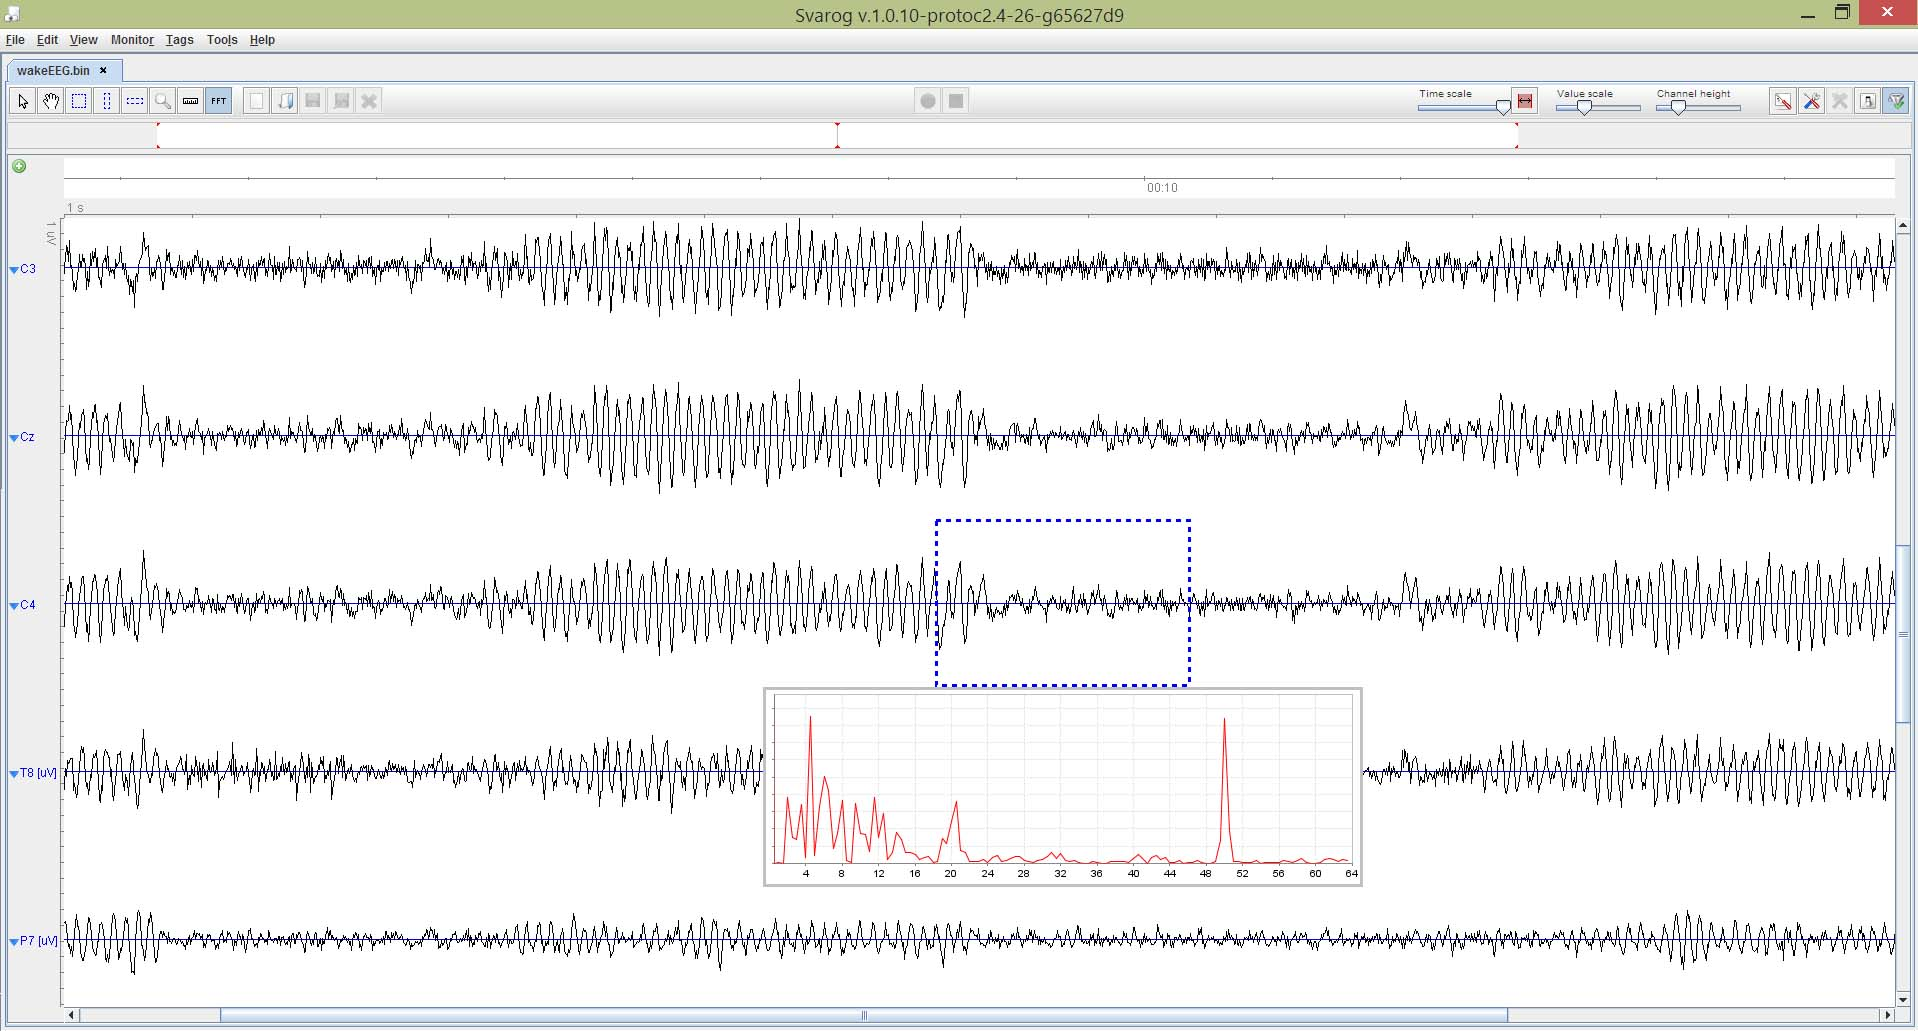
\includegraphics[width=0.8\linewidth]{fig/svarog.jpg}
	\caption{Svarog's main window}
	\label{fig:svarog}
\end{figure}

\section{SigViewer}
SigViewer is a viewing application for biosignals designed to display EEG and other biosignal data. It also supports creating annotations to select artifacts or specific events. Furthermore, it features signal processing modules such as the average over selected epochs and the power spectrum of selected signals. 

The main window has a large area that is composed of individual charts for each signal. The chart can be vertically scrolled and zoomed independently of others, which is useful as waveforms have often very different shape. The annotation tool allows annotations to be created directly over the waveforms and right click on the annotation provides next options. The responsiveness somewhat degrades with too many displayed signals, probably because the plots are rendered in software. SigViewer is implemented in C++ and Qt.

\begin{figure}[htb]
	\centering
	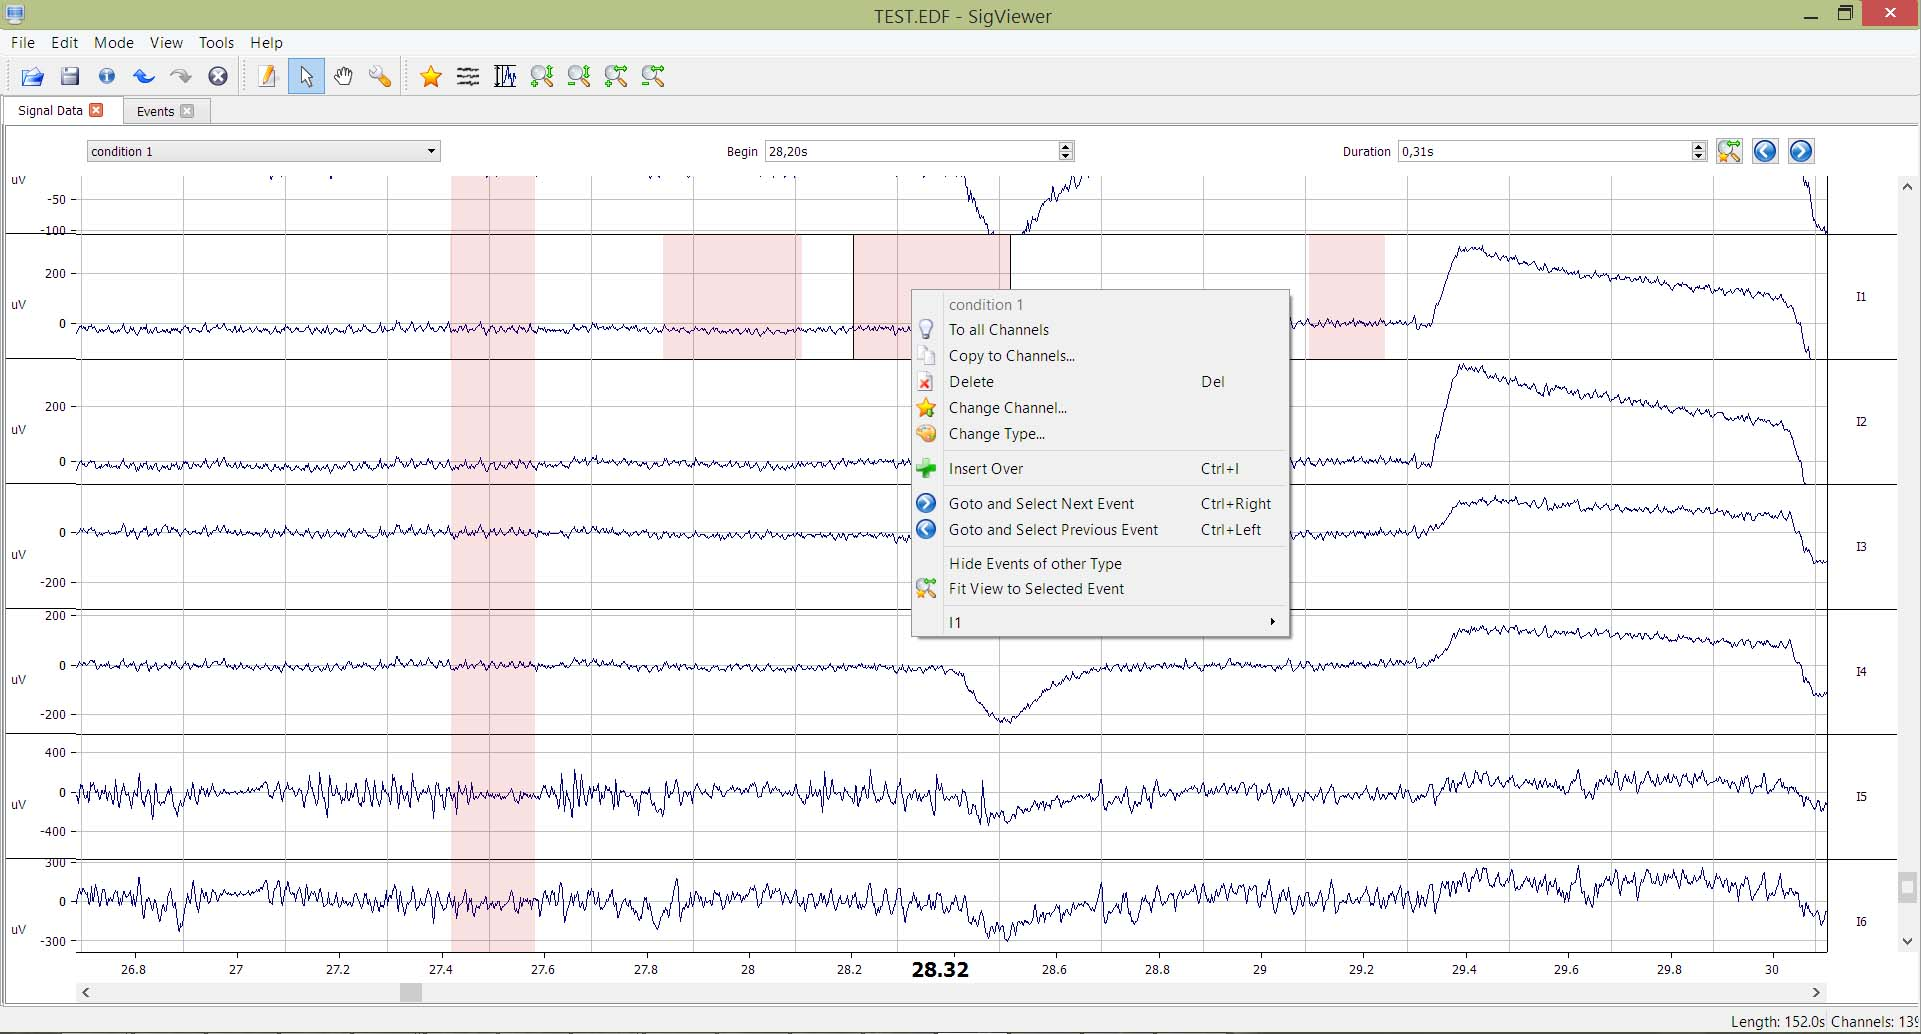
\includegraphics[width=0.8\linewidth]{fig/sigviewer.jpg}
	\caption{SigViewer's main window}
	\label{fig:sigviewer}
\end{figure}

\section{Comparison of Solutions}
The analyzed solutions are diverse enough so that comparison can be made. From the targeted audience view point, it is noticeable that Emotiv software package with all its games and visualization tools targets casual users that are not so much interested in signal analysis, but in the utilization of a brain-computer interface for various tasks. On the other hand, Svarog and SigViewer are more suitable for data analysis. Svarog is a more feature complete and sophisticated application than SigViewer. However, the SigViewer's signal browser, which is the most important element in both applications, is much more convenient to use and the signals are easier to interpret. Table \ref{t:comparison} provides a short summary of features for each solution. 

\begin{table}[htbp]
	\centering
	\begin{tabular}{|c|c|c|c|}
		\hline  & Emotiv & Svarog & SigViewer \\ 
		\hline Recording Support & Yes & Yes & No \\ 
		\hline Signal Browser & Limited & Yes & Yes \\ 
		\hline Visual Electrode Maps & Yes & No & No \\ 
		\hline Annotation Support & No & Yes & Yes \\ 
		\hline Open Source & No & Yes (GPL) & Yes (GPL) \\ 
		\hline 
	\end{tabular} 
	\caption{Comparison of solutions}
	\label{t:comparison}
\end{table}

\chapter{Concept and Design} \label{concept}
It is usually a good idea to create a concept before implementing a non-trivial project. A concept development process helps to make clear which are the important parts of the project and how they are going to communicate and work together to provide desired results. The concept also helps to maintain a good code structure and class hierarchy. Therefore, the text in this chapter defines the concept that will be used during development of the application. Unless explicitly stated otherwise, the term application will further refer to a program that has been developed as a practical part of this thesis. 

\section{Logical Division}
The first step in concept creation is to analyze the problem and divide it into smaller ones. It is possible to split the whole application into individual subsystems:
\begin{itemize}
	\item GUI
	\item Model importer
	\item 3D math library 
	\item Signal input module
	\item Signal processing module
	\item Rendering system
	\item Animation system
\end{itemize}

The following sections will address each subsystem individually.
\subsection{User Interface}
A user interface provides both a user input to the application and an output or feedback from the application. The graphical user interface (\gls{gui}) is a user interfaced composed of graphical elements, such as windows, buttons, text areas, scrollbars, etc. The elements can be grouped and create layouts that are visually appealing. 

An important question to ask is who will be the target audience. The difference between targeting ordinary users and researchers can be seen in Chapter \ref{existSol}. For example. The original assignment predetermines this work to be used primarily for academic purposes. Nevertheless, the ideas of visually appealing graphical elements and friendly user interface will be also incorporated as they can dramatically improve the experience.

A common approach to GUI design is to first create a simple model called mockup. The mockup can be drawn on paper or created using a specialized software. It should capture all the important elements and define their position and purpose. The GUI is then created to resemble the mockup using a technique that is specific to a platform. Section \ref{sec:GUI} presents GUI that was created for application. 

\subsection{Model Importer}
Loading \gls{3d} mesh models into a memory in a representation that may be used for rendering is a non-trivial task. This is further complicated by the diversity of file formats that are used to store \gls{3d} models. One of the most popular file formats is \texttt{Wavefront .obj} file. It can store whole scenes with multiple objects that are represented using polygons. Most of the \gls{3d} modeling software also allows exporting the model composed solely of the triangles that can be rendered directly by OpenGL. Another advantage of the \texttt{Wavefront .obj} file format is that it uses ASCII and human readable data representation. The Listing \ref{lst:ObjFile} shows an example of \texttt{.obj} file that defines a triangle. Due to the stated properties, the format was chosen to store the model of brain. The model of brain was provided by the \emph{Brain for Blender} project\footnote{\url{http://brainder.org/download/brain-for-blender/}}. This brain is an \gls{mri} scan of a real human brain.

\lstset{captionpos=b, caption=The .obj file example, label=lst:ObjFile}
\begin{lstlisting}
	# object Triangle
	v  -0.5 0 0
	v  0.5 0 0
	v  0.25 0.5 0
	# 3 vertices
	
	g Triangle
	f 1 2 3 
	# 1 face
\end{lstlisting}

A model importer has to be able to open \texttt{.obj} file, list stored objects, and provide data for each of them. The data, such as vertex positions, are then passed to rendering system that will render the objects. A \emph{Tiny obj loader}\footnote{\url{http://syoyo.github.io/tinyobjloader/}} library is a perfect solution for our needs. It is light-weight C++ library implemented by single file that is simply compiled with the rest of the application and has no dependencies except for C++ STL. After loading the triangulated model from \texttt{.obj} file, the geometry and other information is conveniently stored inside STL \texttt{vector} that can be used directly by rendering system.

\subsection{3D Math Library}
A \gls{3d} math library is required in order to manipulate objects in \gls{3d} space. Minimal requirement is a support for translation, rotation and projection is needed. The library should also include algorithms for creating transformation matrices used by OpenGL. Naturally, the data structures such as vectors, matrices, and basic geometry should be part of the library.

The \emph{OpenGL Mathematics}\footnote{\url{http://glm.g-truc.net/0.9.6/index.html}} library covers most of these requirements. It provides the same functionality and data types that are found in the GLSL language plus additional useful features such as the matrix transformations, quaternions, data packing, etc. The only drawback is that the library does not provide any \gls{2d} or \gls{3d} objects. Therefore, the application will have to implement these as needed. 

\subsection{Signal Input Module}
The \gls{eeg} data is required by the application in order to produce actual results. The problem is that there are many file formats actively used, some of which are specific to a single medical laboratory or recording equipment. However, there is an effort to create single standard file format. The European Data Format (EDF) is an example of such effort. This format stores electrode signals in form of data records which are time-continuous blocks of samples. The electrode signal may consist of multiple data records and each data record has specified start time. Therefore, the data records may not be contiguous, resulting in a sparse recording. The format also provides additional information, such as duration of the data record and duration of the whole file, maximum and minimum of the signal amplitude, information about a patient, etc. \cite{edfFormat}. 

The EDF format was chosen to be a primary source of \gls{eeg} data because of its popularity and versatility. However, the data format is not trivial to read. Because of this, an already existing C library was used. The \emph{EDFlib}\footnote{\url{http://www.teuniz.net/edflib/}} library supports not only the original EDF format but also its extension EDF+ and derivations BDF and BDF+. The library has also some limitations, such as that the files must be continuous. In other words, sparse recordings are not supported. However, discontinuous files can be converted to continuous files with \emph{EDFbrowser}\footnote{\url{http://www.teuniz.net/edfbrowser/}}. After opening a file in the EDF format, each signal can be read individually as a stream. The signal input module then provides the data to the rest of the application in an internal format.

\subsection{Signal Processing Module}
The signal processing module implements filters and transformations presented in Section \ref{sec:sigProc}. As discussed in that section, the discrete Fourier transform is usually implemented as the fast Fourier transform. There are already many libraries implementing \gls{fft}. One such library is \emph{Kiss FFT}\footnote{\url{http://sourceforge.net/projects/kissfft/}} and it was chosen due to its simplicity, compact size, and benevolent license. However, no simple library could be found that implements FIR filters. It was decided the few filters that are necessary will be implemented anew, rather than including large digital signal processing \gls{dsp} library with lots of dependencies. Section \ref{sec:implFIRfilters} provides implementation details for these filters.

\subsection{Rendering System}
The rendering system provides a necessary functionality to produce a visual output. It is the most complex part of application and can be further divided into:
\begin{itemize}
	\item General rendering support for OpenGL primitives
	\item 3D mesh object rendering support
	\item Electrode visualization
	\item \gls{eeg} data visualization
\end{itemize}

The whole rendering system is hardware accelerated in order to provide a good performance. The hardware acceleration is provided by the OpenGL \gls{api} and graphics pipeline introduced in Section \ref{sec:pipeline}. Because of that, a shader program is needed for each rendering task. The implementations details of shader programs are discussed in Section \ref{sec:implRendering}. 

A \emph{Unishader}\footnote{\url{https://github.com/BetaRavener/UniShader}} library is used to load and utilize the shader programs. The Unishader is previous work by authors of this thesis that creates an automatized wrapper around OpenGL focusing on the shader support. It greatly simplifies the setup and rendering using shader programs. For example, it can automatically query a shader variable type and use appropriate functions, compile and link programs when needed, perform configuration checks, and manage GPU resources. It also helps to keep OpenGL context in a valid state, which is a non trivial task that requires tracking of all the performed operations.

\subsection{Animation System}
\label{ssec:concAnimSystem}
The animation system prepares the \gls{eeg} data for visualization. The system resembles a media player that can play, pause and rewind the content, in this case \gls{eeg} data. However, the amplitude of signal still needs to be somehow transformed into visual information. It was decided that the color of electrode will be used to represent the amplitude. The green color is used for zero amplitude. The maximum positive amplitude is represented by red and negative amplitude by blue color. The resulting gradient is shown in Figure \ref{fig:ElColorGradient}. If no signal is assigned to the electrode it remains gray. A purple color is used if there is not enough data available. The section \ref{sec:animSystem} describes the conversion of signal data to the color in more detail.

\begin{figure}[htb]
	\centering
	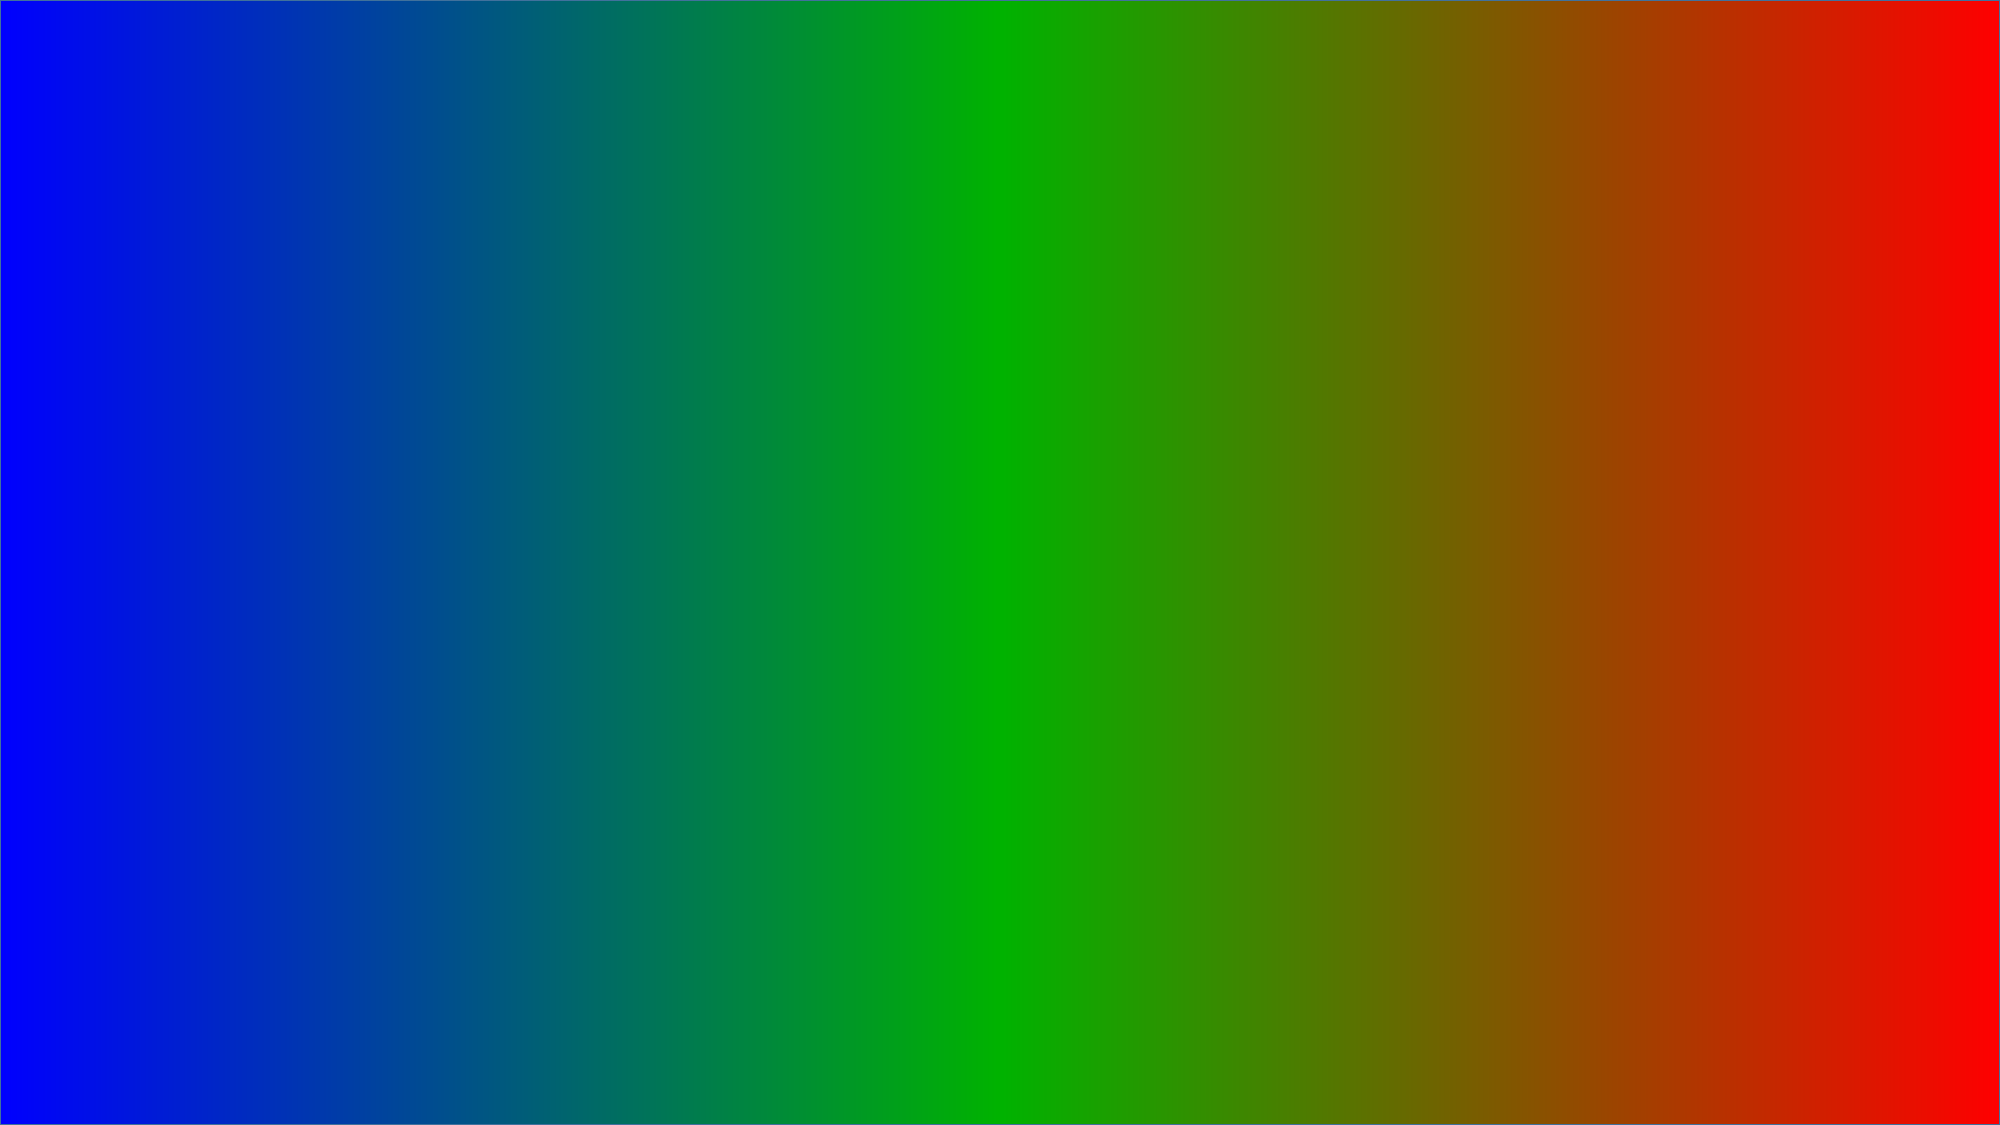
\includegraphics[width=0.8\linewidth, height=0.05\textheight]{fig/gradient.pdf}
	\caption{Electrode color gradient}
	\label{fig:ElColorGradient}
\end{figure}

\chapter{Implementation}
\label{implementation}
This chapter provides more details about significant algorithms and methods used during  development of application. The information provided here is still at some level of abstraction 
so that the algorithms can be understood without knowledge of a specific programming language. 

\section{FIR Filters}
\label{sec:implFIRfilters}
As discussed in Section \ref{sec:sigProc}, the filtering is done by convolution of the input signal with a filter's impulse response. The filter's impulse response is computed directly from the equations presented in Section \ref{ssec:FIRandIIR}. To implement convolution, a sliding window of predefined length is first created. The order of the filter determines the length of the sliding window. The sliding window moves over the signal and at each step it is filled by values it covers. The values are then multiplied by the filter's impulse response and window function coefficients. The values are summed and stored as a single element in a new, filtered sequence. The process is illustrated by Figure \ref{fig:ImplFilter}.

%TODO: Calculate correct output value in the image
\begin{figure}[htb]
	\centering
	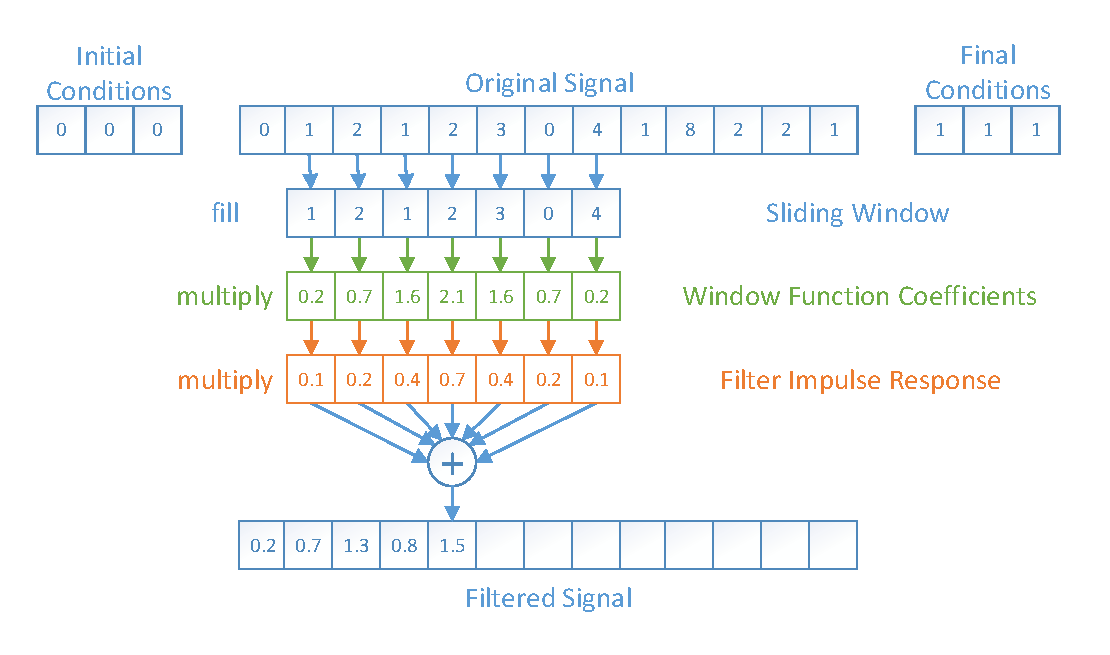
\includegraphics[width=1\linewidth]{fig/implFilter.pdf}
	\caption{Illustration of signal filtering}
	\label{fig:ImplFilter}
\end{figure}

However, there is a problem at the beginning and end of the input signal because there are not enough values to fill the sliding window. This is solved by prepending and appending the input sequence with initial and final conditions respectively. These are short sequences that are generated for each signal individually before it is processed. They may be just filled with zeros, repeat the value at the edge of the signal, or copy the signal values in reversed order. The choice usually depends on the type of the filter.

In order to test the implementation, the results were compared with MATLAB output. First, a set of testing data was created in plain-text format. This data was then processed by the implementation described here using multiple combinations of cut off frequencies, window lengths and window functions. The output was stored in a new file and compared to the output produced by MATLAB filters with the same configuration. The difference between the two was only marginal and can be attributed to floating point errors.

\section{Electrode Placement}
\label{sec:implElPlacement}
It is possible to use a custom layout and electrode labels by importing \texttt{Electrode map file}. The structure of file is simple with a single line header as a first line that is used to check compatibility. The rest of the file are tuples of an electrode name, a \gls{2d} position, and a \gls{3d} position. Each tuple specifies a single electrode. If an electrode position is unknown or was not supplied, it may be omitted by using \texttt{*} . An example of such file is shown in Listing \ref{lst:ElMap}.

\lstset{captionpos=b, caption=Electrode map file example, label=lst:ElMap}
\begin{lstlisting}
    Electrode map file v100
    AF1 -5.91481 30.148 16.8014 24.7601 98.6503
    AF10 29.3892 40.4509 *
    AF2 5.9148 30.148 -17.1713 24.3079 98.5821
\end{lstlisting}

If there is a file \texttt{default.elmap} present inside \texttt{electrodes} folder during the application startup, it will be used to load electrode positions. Otherwise, electrodes will be named according to the 10-10 electrode placement system presented in Section \ref{ssec:elPlacement} and \gls{2d} positions will be generated by program but no \gls{3d} positions will be available because automatic \gls{3d} placement is not supported. The \gls{2d} layout tries to resemble those found in scientific papers. The \gls{3d} positions may be additionally loaded from \texttt{.obj} file. The objects inside this file must be named after electrodes so mapping can be made. The shape of the object doesn't matter as long as the object's center of gravity is in desired position. The Figure \ref{fig:3DSMaxPlacement} illustrates this process using Autodesk 3ds Max. 
\begin{enumerate}
	\item The brain model that is used in application is imported to 3ds Max.
	\item The model of brain is then fitted by a model of skull\footnote{\url{http://www.sharecg.com/get_file.php?upload_file_id=43787&PSID=7e83ca0fc9bc28c873e73f17939f7b13}} that provides features necessary for electrode placement, such as nassion, inion, and auricular points.
	\item The important contours are marked according to Section \ref{ssec:elPlacement} and objects, in this case boxes, are spaced evenly along the contours. The contour is obtained by slicing the skull with a plane that passes through marked points. 
	\item The objects are named after the electrodes.
	\item \texttt{electrodes.obj} file is exported from 3ds Max.
\end{enumerate}
This file can be imported into application to provide \gls{3d} electrode positions.

\begin{figure}[htb]
	\centering
	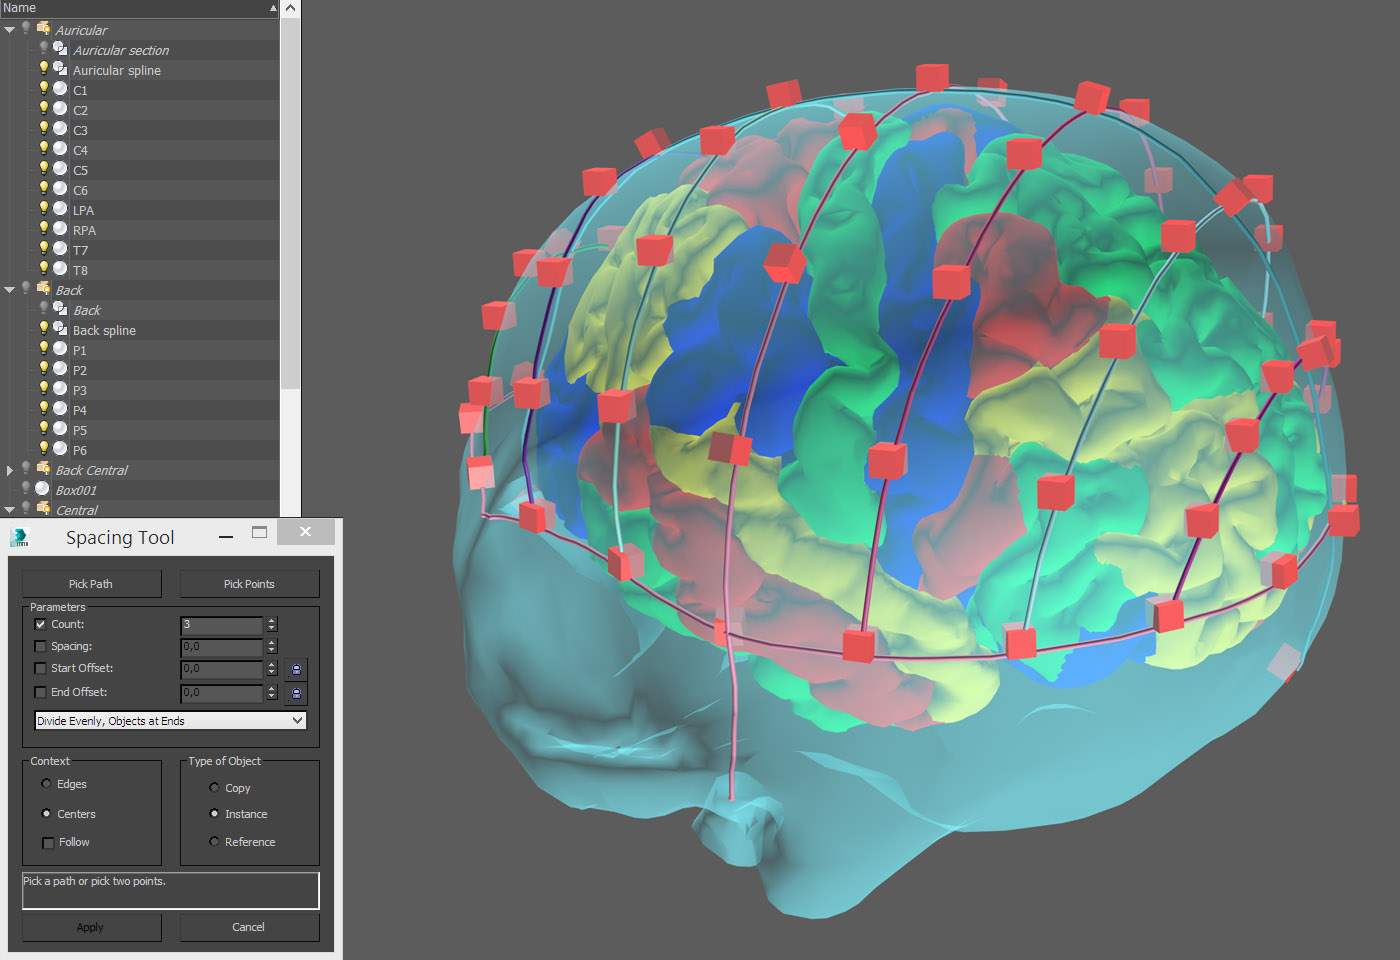
\includegraphics[width=1\linewidth]{fig/3DSMaxPlacement.jpg}
	\caption{Electrode placement in 3ds Max}
	\label{fig:3DSMaxPlacement}
\end{figure}

\section{Rendering System}
\label{sec:implRendering}
All the rendering tasks are hardware accelerated using OpenGL in order to provide a reasonable performance. Because OpenGL is only a low level API, a group of shader programs had to be developed to provide required rendering support. The first shader program allows shaded mesh objects to be rendered in a \gls{3d} space. A shader program that is used for electrode visualization is described in Section \ref{ssec:implElVis}. Another shader program provides functionality to render signals in time domain using lines with custom thickness. More details about this shader program are provided in Section \ref{ssec:ChartView}. Finally, a general purpose shader program for rendering \gls{2d} geometry is included that can be used to render miscellaneous objects in orthogonal projection.  

\subsection{Electrode Visualization}
\label{ssec:implElVis}
The visual appearance of electrodes should resemble an illuminated sphere. Normally this would be done by creating a mesh of the sphere that could be rendered the usual way. However, in order to save memory and to demonstrate capabilities of shader programs, we used a different approach. The input to the shader program consists only of a sphere center position, a color, and a radius. The vertex shader passes the data unaltered to geometry shader. The geometry shader then generates a triangle fan around the center position that is always directed towards the camera. The number of triangles in the fan is variable and when high enough, the fan starts to resemble a circle. The result is then passed to the fragment shader that applies Phong shading. The shading gives a \gls{3d} effect to the circle which now looks like a sphere. Figure \ref{fig:ElRender} illustrates the described rendering process.
%TODO: If not enough, describe phong shading

\begin{figure}[htb]
	\centering
	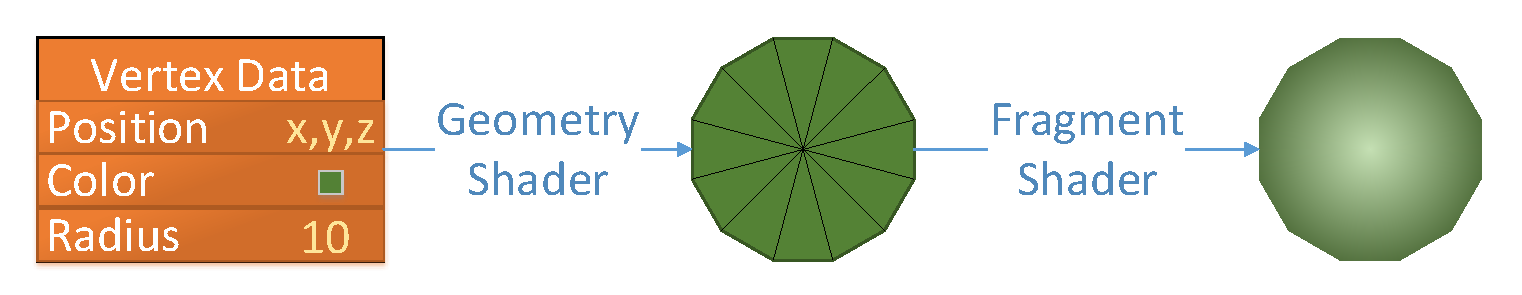
\includegraphics[width=1\linewidth]{fig/ElRender.pdf}
	\caption{Electrode rendering process}
	\label{fig:ElRender}
\end{figure}

\subsection{Chart View}
\label{ssec:ChartView}
The chart view is used primarily to display \gls{eeg} signals in a time domain. The view can be zoomed horizontally to control displayed duration. A vertical zoom is also supported so that the number of signals displayed in the view can be changed. However, the amount of data from an ordinary \gls{eeg} measurement is fairly large. 10 minutes of recording at sampling frequency of \SI{200}{\Hz} produces 120000 samples for each electrode. Rendering so much data would be a very demanding task. Moreover, let's consider a FullHD computer monitor with horizontal resolution of 1920 pixels and a chart view that is fully zoomed out. In this case, approximately 63 samples map to each monitor column, which is obviously redundant.

A solution to this problem is a signal decimation. The most simple way to decimate a signal is to take each N-th sample. However, this would produce very poor results. A better method is to find maximum and minimum value from the samples that would map to the same monitor column and render both of them. While this method is more computationally demanding than just taking N-th sample, it is still much more efficient than rendering all of the data and preserves the shape of the signal. The difference between an original signal and a signal decimated using N-th sample and Min-Max method can be seen in Figure \ref{fig:SignalDecimation}. The decimated signal contains in both cases 100 times less samples than original signal. The decimation was performed on the actual \gls{eeg} data. To optimize even further, the signal decimation is performed only when horizontal zoom changes and the result for that zoom level is cached. This allows scrolling the view swiftly without any further preprocessing.
\begin{figure}[htb]
	\centering
	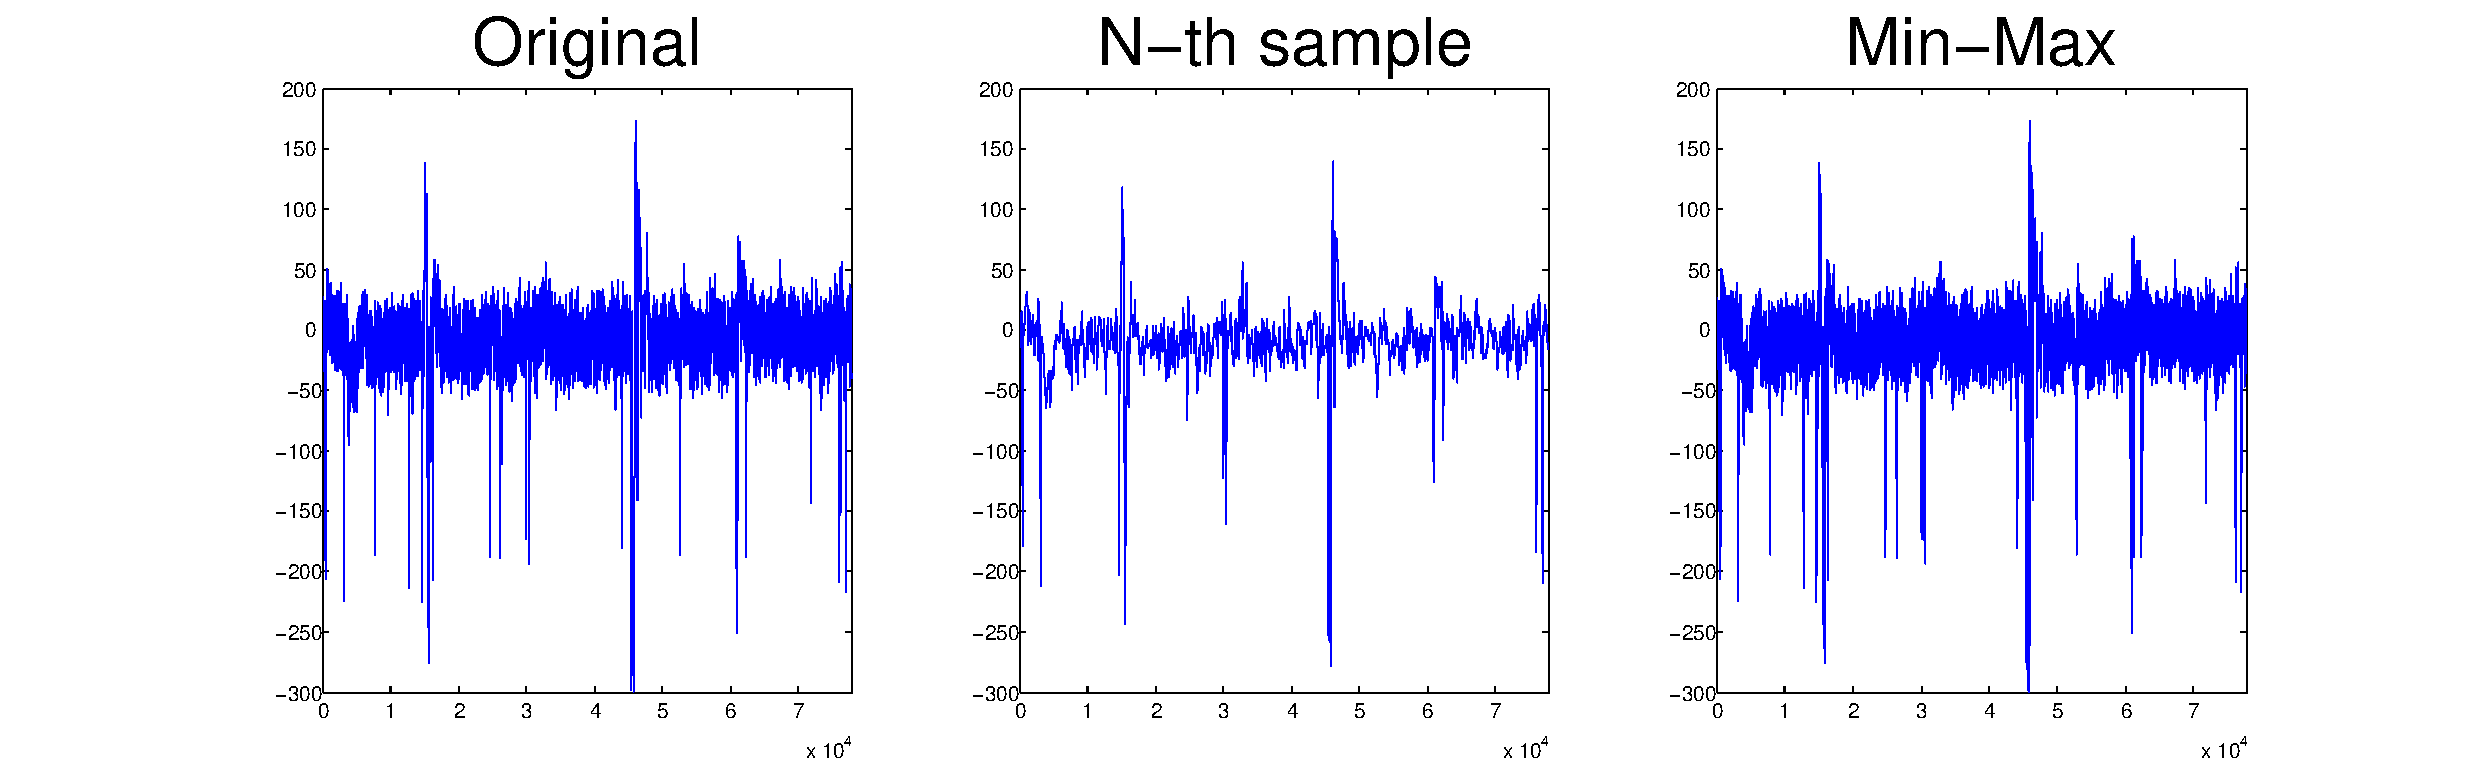
\includegraphics[width=1\linewidth]{fig/signalDec.pdf}
	\caption{The original and decimated signals}
	\label{fig:SignalDecimation}
\end{figure}
This approach can be also used for real-time recording when data are not static. A newly recorded sample is simply appended to the signal and only last value of cache needs to be updated.  

The decimated signal can be finally rendered using a specialized shader program. The main feature of this shader program is the support for rendering lines with specified thickness. This must be done by generating two triangles for each line in a geometry shader because OpenGL can draw only lines without thickness. However, this produces gaps between lines as the slope changes. In order to render a smooth, continuous curve, the geometry shader also creates capped line joins. Figure \ref{fig:LinesAndJoin} illustrates the situation where the points A, B, and C are the samples that define two lines. Furthermore, each signal has designated area for drawing to prevent overlaps which are confusing when analyzing data. A pixel that is produced outside of this area is discarded by fragment shader.

\begin{figure}[htb]
	\centering
	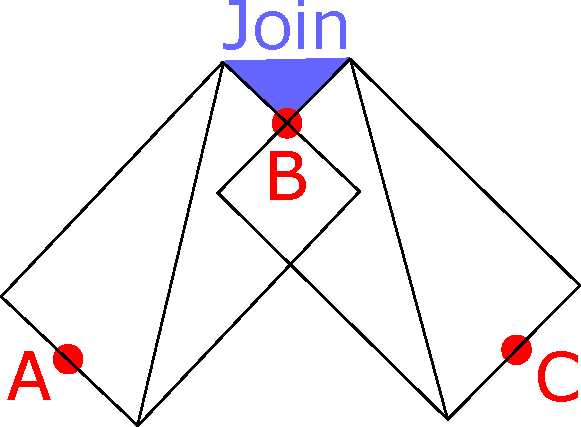
\includegraphics[width=0.6\linewidth, height=0.2\textheight]{fig/linesAndJoin.pdf}
	\caption{The lines with a thickness and a capped line join}
	\label{fig:LinesAndJoin}
\end{figure}

\section{Animation of Electrodes}
\label{sec:animSystem}
The electrodes are animated by changing their color over time. The electrode remains gray if there is no signal assigned. Otherwise, a normalized value in range from -1 to 1 determines the color of the electrode using gradient presented in \ref{ssec:concAnimSystem}. A user can choose between two animation modes. The first one produces normalized value directly by dividing the amplitude of the signal at the current animation time by the maximum signal amplitude range according to Equation \ref{eq:xNorm}. The second mode uses \gls{fft} to obtain the spectrum of the signal around the current animation time. The user can specify frequency range that will be analyzed. A frequency component with maximum amplitude over this range is then selected and normalized. The electrode color turns purple if there is not enough data to perform \gls{fft}. Because most of the time the signal amplitude is much lower than maximum amplitude, a gain factor can be specified. The normalized value is multiplied by this factor and the result is clamped back to the allowed range.

\begin{equation}
\label{eq:xNorm}
x_{norm} = \frac{x - x_{min}}{x_{max} - x_{min}}
\end{equation}

\section{Graphical User Interface}
\label{sec:GUI}
The application user interface was created with emphasis on simplicity and clean look. When the application is executed, only a main window appears. Its dominant element is the chart view described in Section \ref{ssec:ChartView} and displayed in Figure \ref{fig:chartView}. The main window features only two more buttons for playing and rewinding the animation. The current animation time is shown in the chart as a yellow line. Using a right mouse button over the chart moves the line into the mouse position and sets the animation time accordingly. The main window menu bar gives access to additional dialogs and windows:

\begin{figure}[htb]
	\centering
	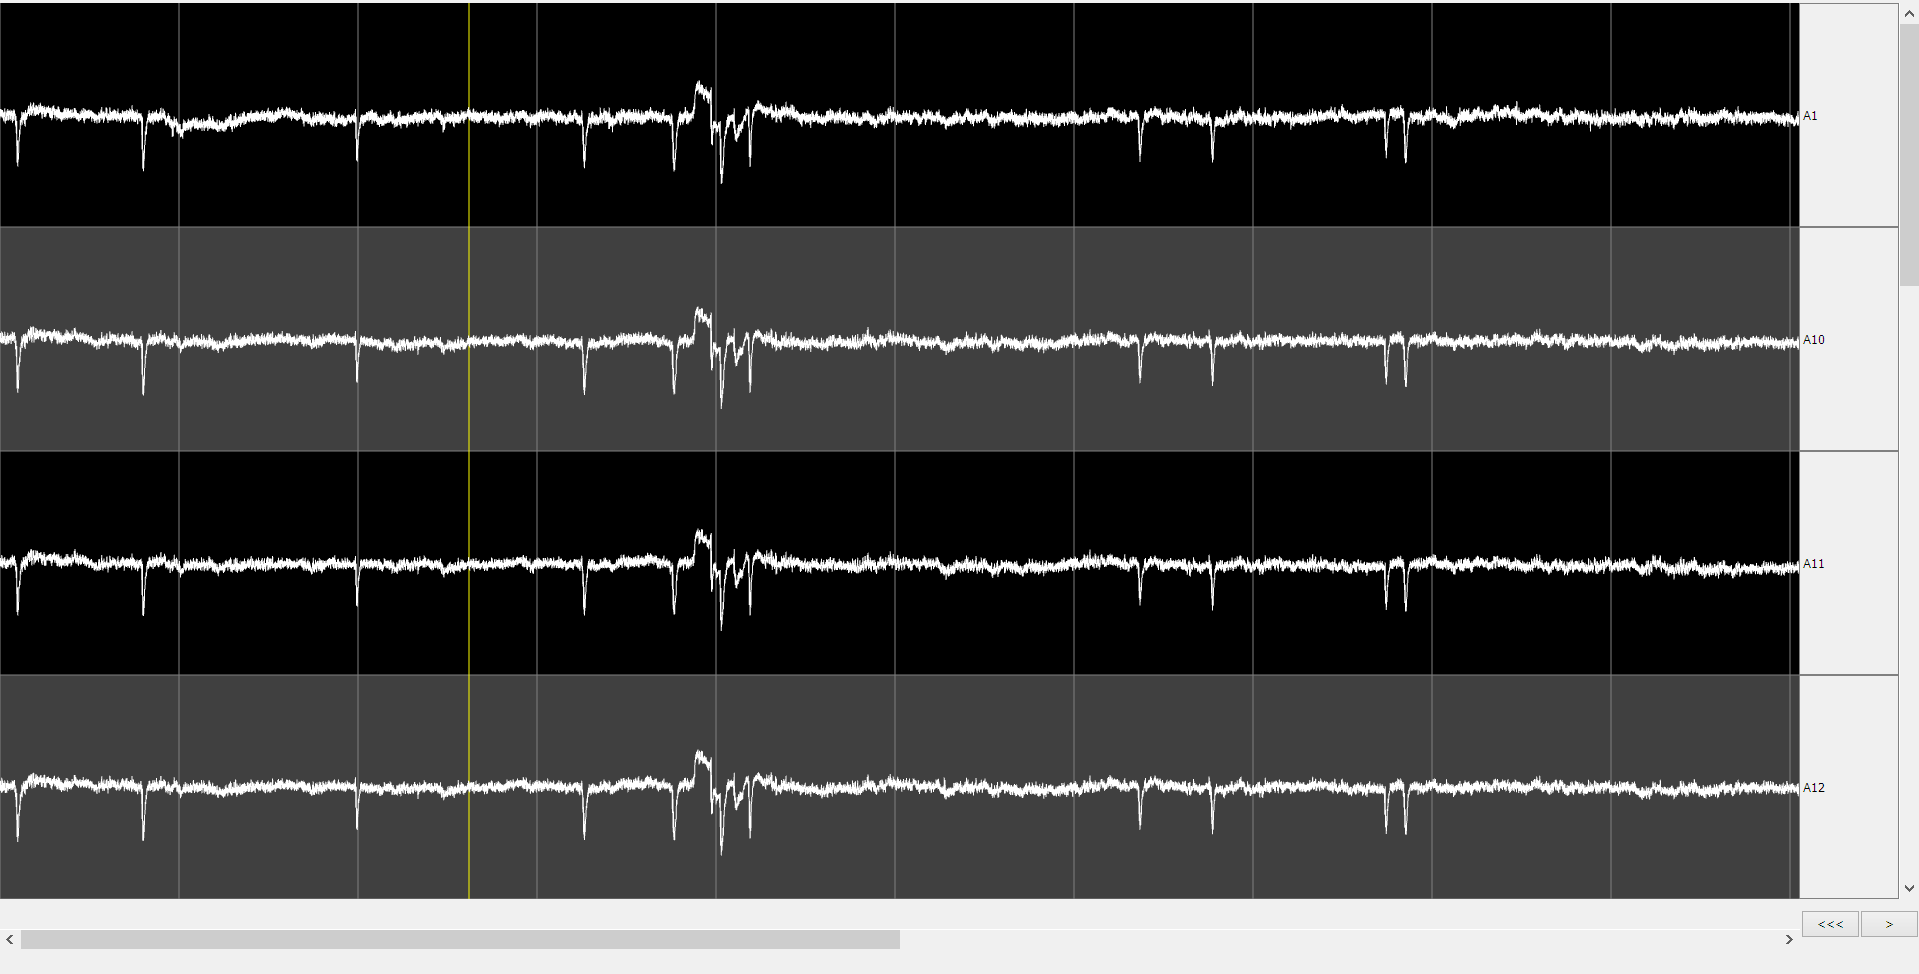
\includegraphics[width=1\linewidth]{fig/chartView.png}
	\caption{Chart view}
	\label{fig:chartView}
\end{figure}

\begin{description}
	\item[Open signal file dialog] provides interface for opening a file with data and listing available signals. The user then selects which records he wants to work with by moving them into the second list. The labels used for records in the file may not conform to names used for electrodes in the electrode placement system. To address this, the user can assign the electrode to each recording manually. However, if the electrode and data record labels match, an auto-assignment button can be used to pair them. The electrode assignments can be exported to a file and imported later as needed.
	
	\item[Electrode map dialog] allows importing and exporting electrode map files. It also allows electrode positions to be set using \texttt{.obj} file as described in Section \ref{sec:implElPlacement}.
	
	\item[Filter dialog] provides an interface to the signal filtering. It allows choosing between the low pass and high pass filter and specifying the cutoff frequency, window function, and length of the window. The dialog also provides feedback on progress in form of a progress bar as the filtering operation can take a long time to finish.
	
	\item[Player settings dialog] allows the animation settings to be modified. The gain factor introduced in Section \ref{sec:animSystem}, refresh rate, and animation speed can be changed here. The user can also select the transformation used by animation and specify the frequency range. Changes to this dialog are applied immediately to make it easier to experiment with different values.
	
	\item[Electrode 2D and 3D view] can be displayed, each in its own window. Both views can be manipulated using mouse. The panning can be done by moving the mouse while holding the right mouse button and using the scroll wheel the user can zoom in and out. In the \gls{3d} view the user can also rotate the view by holding the left mouse button. Figures \ref{fig:view2D} and \ref{fig:view3D} show the \gls{2d} and \gls{3d} view respectively.
\end{description}

\begin{figure}[htb]
	\centering
	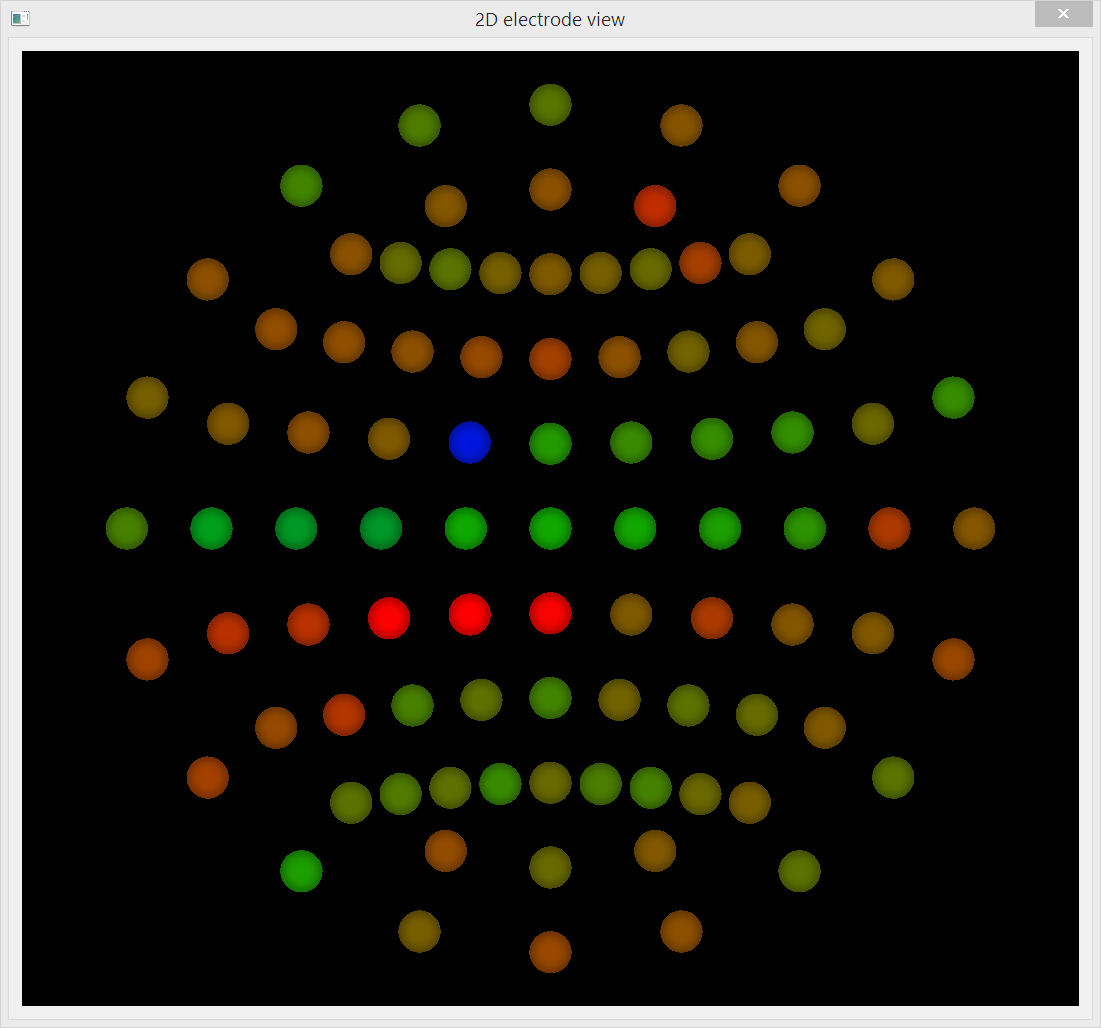
\includegraphics[width=0.7\linewidth]{fig/view2D.png}
	\caption{Electrode 2D view}
	\label{fig:view2D}
\end{figure}

\begin{figure}[htb]
	\centering
	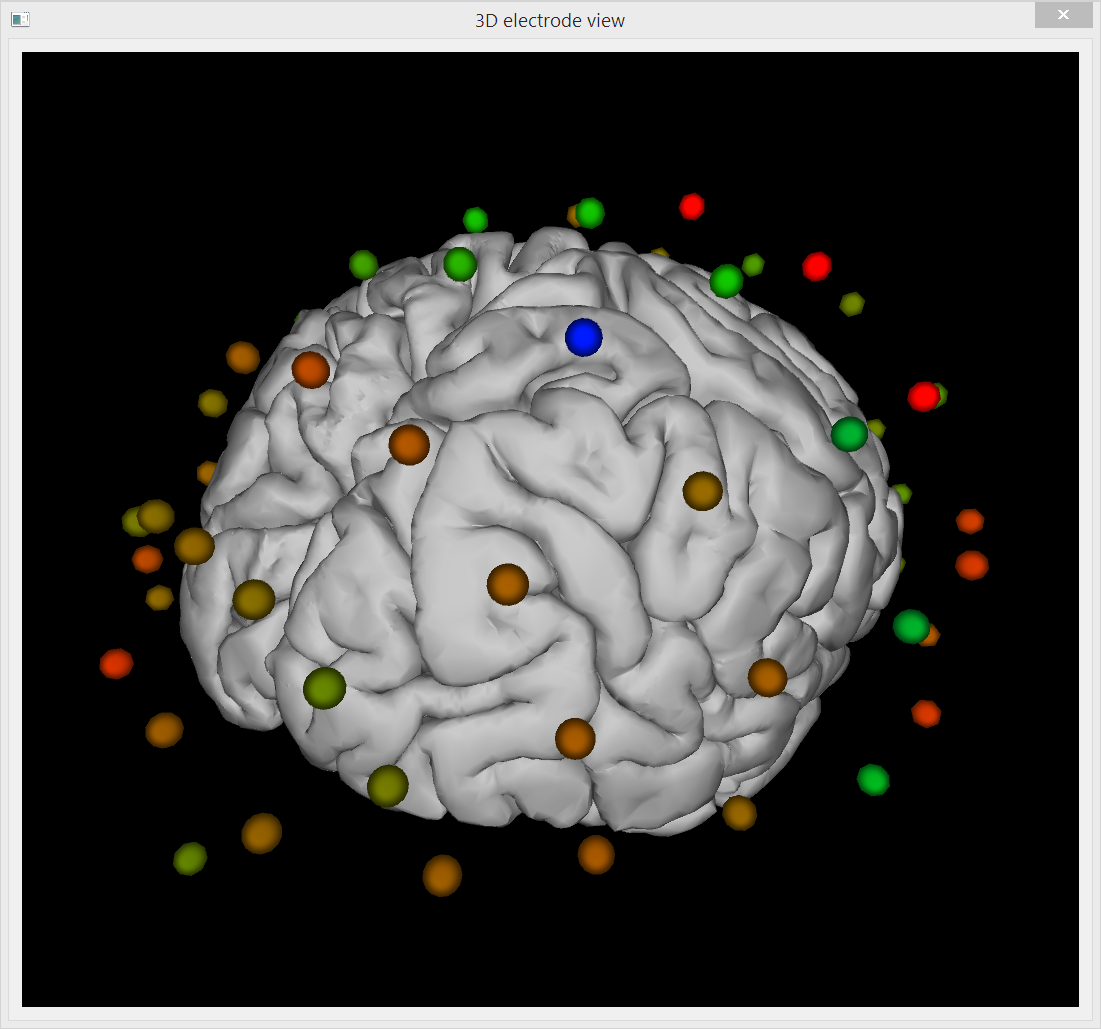
\includegraphics[width=0.7\linewidth]{fig/view3D.png}
	\caption{Electrode 3D view}
	\label{fig:view3D}
\end{figure}

%\chapter{Results}
%Summarization of results obtained by this work, final graphs and tables,
%higlighting of the most interesting parts, presentation of user 
%research -- opinions, suggestions,
%feture requests..
%\chapter{Discussion}
%Discussing the results in regard to referenced literature and their results.
%Showing significance of findings, questioning them, providing several
%perspectives and means for argumentation.

\chapter{Conclusion and Future Directions}
This work provides a brief introduction to a human brain. It also describes
neuronal activity that occurs within the brain and methods for measuring this activity, specifically EEG. The EEG is presented in more detail as this work is concerned with visualization of data obtained by this technology. First, the basic principles of EEG and measuring equipment are described. Moving on, an information about electrode placement is provided, which was important later for correct electrode positioning. Finally, a general measurement procedure and following data analysis is briefly described. This work also provides information about basic methods of signal processing, such as DFT and signal filtering, and presents modern techniques of data visualization using GPU accelerated shader programs.

Following the theoretical background, a concept for a computer application that visualizes brain signals measured by EEG, is presented. The concept builds upon previously analyzed applications created by other individuals or companies. Finally, significant algorithms along with solutions to problems that arose during implementation are described. One such problem was that the amount of data produced by EEG recording was large and had to be optimized in order to provide a reasonable performance. The performance had to be considered also when designing the signal processing module as it encompasses demanding operations.

All rendering tasks are hardware accelerated by GPU. Therefore, the host application had to be accompanied also with shader programs that can render brain, electrodes, signal waveforms and other visual elements. The hardware acceleration allows large data sets and models to be rendered in quality that would not be possible with software rendering. 

The application was formerly designed as both an online and an offline data visualizer. However, only the offline part was implemented due to complications with real-time signal processing and unavailability of recording equipment. Therefore, the plans for the future development include the real-time input module and modification of signal processing algorithms. Other than that, the application could benefit from a wider range of data processing tools and visualization methods, such as frequency spectrum chart that could display result of FFT.

%TODO: The application tries to provide both a data analysis tool and interactive visualizations. An appplication that would serve both as a data analysis tool and interactive...

%Referring to introduction and checking with goals, if everything required was done, what couldn't be done and why.

%Part about possible plans for future, improvement, enhancements, follow up..
%=========================================================================
 % viz. obsah.tex

  % Pouzita literatura
  % ----------------------------------------------
\ifczech
  \bibliographystyle{czechiso}
\else 
  \bibliographystyle{plain}
%  \bibliographystyle{alpha}
\fi
  \begin{flushleft}
  \bibliography{literatura} % viz. literatura.bib
  \end{flushleft}
  \appendix
  
  %\chapter{Obsah CD}
%\chapter{Manual}
%\chapter{Konfigrační soubor}
%\chapter{RelaxNG Schéma konfiguračního soboru}
%\chapter{Plakat}

 % viz. prilohy.tex
\end{document}
